
%% bare_jrnl_compsoc.tex
%% V1.4b
%% 2015/08/26
%% by Michael Shell
%% See:
%% http://www.michaelshell.org/
%% for current contact information.
%%
%% This is a skeleton file demonstrating the use of IEEEtran.cls
%% (requires IEEEtran.cls version 1.8b or later) with an IEEE
%% Computer Society journal paper.
%%
%% Support sites:
%% http://www.michaelshell.org/tex/ieeetran/
%% http://www.ctan.org/pkg/ieeetran
%% and
%% http://www.ieee.org/

%%*************************************************************************
%% Legal Notice:
%% This code is offered as-is without any warranty either expressed or
%% implied; without even the implied warranty of MERCHANTABILITY or
%% FITNESS FOR A PARTICULAR PURPOSE! 
%% User assumes all risk.
%% In no event shall the IEEE or any contributor to this code be liable for
%% any damages or losses, including, but not limited to, incidental,
%% consequential, or any other damages, resulting from the use or misuse
%% of any information contained here.
%%
%% All comments are the opinions of their respective authors and are not
%% necessarily endorsed by the IEEE.
%%
%% This work is distributed under the LaTeX Project Public License (LPPL)
%% ( http://www.latex-project.org/ ) version 1.3, and may be freely used,
%% distributed and modified. A copy of the LPPL, version 1.3, is included
%% in the base LaTeX documentation of all distributions of LaTeX released
%% 2003/12/01 or later.
%% Retain all contribution notices and credits.
%% ** Modified files should be clearly indicated as such, including  **
%% ** renaming them and changing author support contact information. **
%%*************************************************************************


% *** Authors should verify (and, if needed, correct) their LaTeX system  ***
% *** with the testflow diagnostic prior to trusting their LaTeX platform ***
% *** with production work. The IEEE's font choices and paper sizes can   ***
% *** trigger bugs that do not appear when using other class files.       ***                          ***
% The testflow support page is at:
% http://www.michaelshell.org/tex/testflow/


\documentclass[10pt,journal,compsoc]{IEEEtran}
%
% If IEEEtran.cls has not been installed into the LaTeX system files,
% manually specify the path to it like:
% \documentclass[10pt,journal,compsoc]{../sty/IEEEtran}





% Some very useful LaTeX packages include:
% (uncomment the ones you want to load)


% *** MISC UTILITY PACKAGES ***
%
%\usepackage{ifpdf}
% Heiko Oberdiek's ifpdf.sty is very useful if you need conditional
% compilation based on whether the output is pdf or dvi.
% usage:
% \ifpdf
%   % pdf code
% \else
%   % dvi code
% \fi
% The latest version of ifpdf.sty can be obtained from:
% http://www.ctan.org/pkg/ifpdf
% Also, note that IEEEtran.cls V1.7 and later provides a builtin
% \ifCLASSINFOpdf conditional that works the same way.
% When switching from latex to pdflatex and vice-versa, the compiler may
% have to be run twice to clear warning/error messages.






% *** CITATION PACKAGES ***
%
\ifCLASSOPTIONcompsoc
  % IEEE Computer Society needs nocompress option
  % requires cite.sty v4.0 or later (November 2003)
  \usepackage[nocompress]{cite}
\else
  % normal IEEE
  \usepackage{cite}
\fi
% cite.sty was written by Donald Arseneau
% V1.6 and later of IEEEtran pre-defines the format of the cite.sty package
% \cite{} output to follow that of the IEEE. Loading the cite package will
% result in citation numbers being automatically sorted and properly
% "compressed/ranged". e.g., [1], [9], [2], [7], [5], [6] without using
% cite.sty will become [1], [2], [5]--[7], [9] using cite.sty. cite.sty's
% \cite will automatically add leading space, if needed. Use cite.sty's
% noadjust option (cite.sty V3.8 and later) if you want to turn this off
% such as if a citation ever needs to be enclosed in parenthesis.
% cite.sty is already installed on most LaTeX systems. Be sure and use
% version 5.0 (2009-03-20) and later if using hyperref.sty.
% The latest version can be obtained at:
% http://www.ctan.org/pkg/cite
% The documentation is contained in the cite.sty file itself.
%
% Note that some packages require special options to format as the Computer
% Society requires. In particular, Computer Society  papers do not use
% compressed citation ranges as is done in typical IEEE papers
% (e.g., [1]-[4]). Instead, they list every citation separately in order
% (e.g., [1], [2], [3], [4]). To get the latter we need to load the cite
% package with the nocompress option which is supported by cite.sty v4.0
% and later. Note also the use of a CLASSOPTION conditional provided by
% IEEEtran.cls V1.7 and later.





% *** GRAPHICS RELATED PACKAGES ***
%
\ifCLASSINFOpdf
  % \usepackage[pdftex]{graphicx}
  % declare the path(s) where your graphic files are
  % \graphicspath{{../pdf/}{../jpeg/}}
  % and their extensions so you won't have to specify these with
  % every instance of \includegraphics
  % \DeclareGraphicsExtensions{.pdf,.jpeg,.png}
\else
  % or other class option (dvipsone, dvipdf, if not using dvips). graphicx
  % will default to the driver specified in the system graphics.cfg if no
  % driver is specified.
  % \usepackage[dvips]{graphicx}
  % declare the path(s) where your graphic files are
  % \graphicspath{{../eps/}}
  % and their extensions so you won't have to specify these with
  % every instance of \includegraphics
  % \DeclareGraphicsExtensions{.eps}
\fi
% graphicx was written by David Carlisle and Sebastian Rahtz. It is
% required if you want graphics, photos, etc. graphicx.sty is already
% installed on most LaTeX systems. The latest version and documentation
% can be obtained at: 
% http://www.ctan.org/pkg/graphicx
% Another good source of documentation is "Using Imported Graphics in
% LaTeX2e" by Keith Reckdahl which can be found at:
% http://www.ctan.org/pkg/epslatex
%
% latex, and pdflatex in dvi mode, support graphics in encapsulated
% postscript (.eps) format. pdflatex in pdf mode supports graphics
% in .pdf, .jpeg, .png and .mps (metapost) formats. Users should ensure
% that all non-photo figures use a vector format (.eps, .pdf, .mps) and
% not a bitmapped formats (.jpeg, .png). The IEEE frowns on bitmapped formats
% which can result in "jaggedy"/blurry rendering of lines and letters as
% well as large increases in file sizes.
%
% You can find documentation about the pdfTeX application at:
% http://www.tug.org/applications/pdftex






% *** MATH PACKAGES ***
%
%\usepackage{amsmath}
% A popular package from the American Mathematical Society that provides
% many useful and powerful commands for dealing with mathematics.
%
% Note that the amsmath package sets \interdisplaylinepenalty to 10000
% thus preventing page breaks from occurring within multiline equations. Use:
%\interdisplaylinepenalty=2500
% after loading amsmath to restore such page breaks as IEEEtran.cls normally
% does. amsmath.sty is already installed on most LaTeX systems. The latest
% version and documentation can be obtained at:
% http://www.ctan.org/pkg/amsmath





% *** SPECIALIZED LIST PACKAGES ***
%
%\usepackage{algorithmic}
% algorithmic.sty was written by Peter Williams and Rogerio Brito.
% This package provides an algorithmic environment fo describing algorithms.
% You can use the algorithmic environment in-text or within a figure
% environment to provide for a floating algorithm. Do NOT use the algorithm
% floating environment provided by algorithm.sty (by the same authors) or
% algorithm2e.sty (by Christophe Fiorio) as the IEEE does not use dedicated
% algorithm float types and packages that provide these will not provide
% correct IEEE style captions. The latest version and documentation of
% algorithmic.sty can be obtained at:
% http://www.ctan.org/pkg/algorithms
% Also of interest may be the (relatively newer and more customizable)
% algorithmicx.sty package by Szasz Janos:
% http://www.ctan.org/pkg/algorithmicx




% *** ALIGNMENT PACKAGES ***
%
%\usepackage{array}
% Frank Mittelbach's and David Carlisle's array.sty patches and improves
% the standard LaTeX2e array and tabular environments to provide better
% appearance and additional user controls. As the default LaTeX2e table
% generation code is lacking to the point of almost being broken with
% respect to the quality of the end results, all users are strongly
% advised to use an enhanced (at the very least that provided by array.sty)
% set of table tools. array.sty is already installed on most systems. The
% latest version and documentation can be obtained at:
% http://www.ctan.org/pkg/array


% IEEEtran contains the IEEEeqnarray family of commands that can be used to
% generate multiline equations as well as matrices, tables, etc., of high
% quality.




% *** SUBFIGURE PACKAGES ***
%\ifCLASSOPTIONcompsoc
%  \usepackage[caption=false,font=footnotesize,labelfont=sf,textfont=sf]{subfig}
%\else
%  \usepackage[caption=false,font=footnotesize]{subfig}
%\fi
% subfig.sty, written by Steven Douglas Cochran, is the modern replacement
% for subfigure.sty, the latter of which is no longer maintained and is
% incompatible with some LaTeX packages including fixltx2e. However,
% subfig.sty requires and automatically loads Axel Sommerfeldt's caption.sty
% which will override IEEEtran.cls' handling of captions and this will result
% in non-IEEE style figure/table captions. To prevent this problem, be sure
% and invoke subfig.sty's "caption=false" package option (available since
% subfig.sty version 1.3, 2005/06/28) as this is will preserve IEEEtran.cls
% handling of captions.
% Note that the Computer Society format requires a sans serif font rather
% than the serif font used in traditional IEEE formatting and thus the need
% to invoke different subfig.sty package options depending on whether
% compsoc mode has been enabled.
%
% The latest version and documentation of subfig.sty can be obtained at:
% http://www.ctan.org/pkg/subfig




% *** FLOAT PACKAGES ***
%
%\usepackage{fixltx2e}
% fixltx2e, the successor to the earlier fix2col.sty, was written by
% Frank Mittelbach and David Carlisle. This package corrects a few problems
% in the LaTeX2e kernel, the most notable of which is that in current
% LaTeX2e releases, the ordering of single and double column floats is not
% guaranteed to be preserved. Thus, an unpatched LaTeX2e can allow a
% single column figure to be placed prior to an earlier double column
% figure.
% Be aware that LaTeX2e kernels dated 2015 and later have fixltx2e.sty's
% corrections already built into the system in which case a warning will
% be issued if an attempt is made to load fixltx2e.sty as it is no longer
% needed.
% The latest version and documentation can be found at:
% http://www.ctan.org/pkg/fixltx2e


%\usepackage{stfloats}
% stfloats.sty was written by Sigitas Tolusis. This package gives LaTeX2e
% the ability to do double column floats at the bottom of the page as well
% as the top. (e.g., "\begin{figure*}[!b]" is not normally possible in
% LaTeX2e). It also provides a command:
%\fnbelowfloat
% to enable the placement of footnotes below bottom floats (the standard
% LaTeX2e kernel puts them above bottom floats). This is an invasive package
% which rewrites many portions of the LaTeX2e float routines. It may not work
% with other packages that modify the LaTeX2e float routines. The latest
% version and documentation can be obtained at:
% http://www.ctan.org/pkg/stfloats
% Do not use the stfloats baselinefloat ability as the IEEE does not allow
% \baselineskip to stretch. Authors submitting work to the IEEE should note
% that the IEEE rarely uses double column equations and that authors should try
% to avoid such use. Do not be tempted to use the cuted.sty or midfloat.sty
% packages (also by Sigitas Tolusis) as the IEEE does not format its papers in
% such ways.
% Do not attempt to use stfloats with fixltx2e as they are incompatible.
% Instead, use Morten Hogholm'a dblfloatfix which combines the features
% of both fixltx2e and stfloats:
%
% \usepackage{dblfloatfix}
% The latest version can be found at:
% http://www.ctan.org/pkg/dblfloatfix




%\ifCLASSOPTIONcaptionsoff
%  \usepackage[nomarkers]{endfloat}
% \let\MYoriglatexcaption\caption
% \renewcommand{\caption}[2][\relax]{\MYoriglatexcaption[#2]{#2}}
%\fi
% endfloat.sty was written by James Darrell McCauley, Jeff Goldberg and 
% Axel Sommerfeldt. This package may be useful when used in conjunction with 
% IEEEtran.cls'  captionsoff option. Some IEEE journals/societies require that
% submissions have lists of figures/tables at the end of the paper and that
% figures/tables without any captions are placed on a page by themselves at
% the end of the document. If needed, the draftcls IEEEtran class option or
% \CLASSINPUTbaselinestretch interface can be used to increase the line
% spacing as well. Be sure and use the nomarkers option of endfloat to
% prevent endfloat from "marking" where the figures would have been placed
% in the text. The two hack lines of code above are a slight modification of
% that suggested by in the endfloat docs (section 8.4.1) to ensure that
% the full captions always appear in the list of figures/tables - even if
% the user used the short optional argument of \caption[]{}.
% IEEE papers do not typically make use of \caption[]'s optional argument,
% so this should not be an issue. A similar trick can be used to disable
% captions of packages such as subfig.sty that lack options to turn off
% the subcaptions:
% For subfig.sty:
% \let\MYorigsubfloat\subfloat
% \renewcommand{\subfloat}[2][\relax]{\MYorigsubfloat[]{#2}}
% However, the above trick will not work if both optional arguments of
% the \subfloat command are used. Furthermore, there needs to be a
% description of each subfigure *somewhere* and endfloat does not add
% subfigure captions to its list of figures. Thus, the best approach is to
% avoid the use of subfigure captions (many IEEE journals avoid them anyway)
% and instead reference/explain all the subfigures within the main caption.
% The latest version of endfloat.sty and its documentation can obtained at:
% http://www.ctan.org/pkg/endfloat
%
% The IEEEtran \ifCLASSOPTIONcaptionsoff conditional can also be used
% later in the document, say, to conditionally put the References on a 
% page by themselves.




% *** PDF, URL AND HYPERLINK PACKAGES ***
%
%\usepackage{url}
% url.sty was written by Donald Arseneau. It provides better support for
% handling and breaking URLs. url.sty is already installed on most LaTeX
% systems. The latest version and documentation can be obtained at:
% http://www.ctan.org/pkg/url
% Basically, \url{my_url_here}.





% *** Do not adjust lengths that control margins, column widths, etc. ***
% *** Do not use packages that alter fonts (such as pslatex).         ***
% There should be no need to do such things with IEEEtran.cls V1.6 and later.
% (Unless specifically asked to do so by the journal or conference you plan
% to submit to, of course. )


% correct bad hyphenation here
\hyphenation{op-tical net-works semi-conduc-tor}

\usepackage{cite}
\usepackage{amsmath,amssymb,amsfonts}
\usepackage{algorithmic}
\usepackage{algorithm}
\usepackage{graphicx}
\usepackage{textcomp}
\usepackage{xcolor}

\begin{document}
%
% paper title
% Titles are generally capitalized except for words such as a, an, and, as,
% at, but, by, for, in, nor, of, on, or, the, to and up, which are usually
% not capitalized unless they are the first or last word of the title.
% Linebreaks \\ can be used within to get better formatting as desired.
% Do not put math or special symbols in the title.
\title{Large-Scale Auto K-Means Clustering for Heterogeneous Many-Core Supercomputers}
%
%
% author names and IEEE memberships
% note positions of commas and nonbreaking spaces ( ~ ) LaTeX will not break
% a structure at a ~ so this keeps an author's name from being broken across
% two lines.
% use \thanks{} to gain access to the first footnote area
% a separate \thanks must be used for each paragraph as LaTeX2e's \thanks
% was not built to handle multiple paragraphs
%
%
%\IEEEcompsocitemizethanks is a special \thanks that produces the bulleted
% lists the Computer Society journals use for "first footnote" author
% affiliations. Use \IEEEcompsocthanksitem which works much like \item
% for each affiliation group. When not in compsoc mode,
% \IEEEcompsocitemizethanks becomes like \thanks and
% \IEEEcompsocthanksitem becomes a line break with idention. This
% facilitates dual compilation, although admittedly the differences in the
% desired content of \author between the different types of papers makes a
% one-size-fits-all approach a daunting prospect. For instance, compsoc 
% journal papers have the author affiliations above the "Manuscript
% received ..."  text while in non-compsoc journals this is reversed. Sigh.

\author{Teng Yu,
        Wenlai Zhao,
        Pan Liu,
        Shicai Wang,
        Xiaohan Yan, \\
        Vladimir Janjic,
        Haohuan Fu,
        John Thomson
  %      ~\IEEEmembership{Life~Fellow,~IEEE}% <-this % stops a space
\thanks{This work is an extended version of the paper 'Large-Scale Hierarchical K-Means for Heterogeneous Many-core Supercomputers' that appeared in the 2018 International Conference for High Performance Computing, Networking, Storage and Analysis (SC18) \cite{li2018large}. The additional content includes: 
(i) An auto-learning layer to determine the optimal number of clusters targeting massively large-scale datasets without prior knowledge - Section~\ref{background_J}, Section~\ref{auto-implementation}.
(ii) Experiments on massively gene expression datasets and outperforms the previous research~\cite{wang2014optimising} - Section~\ref{applications}. 
(iii) Adding performance comparisons by Pflops with others approaches - Table 3. 
}  

\IEEEcompsocitemizethanks
{\IEEEcompsocthanksitem T.Yu, V.Janjic and J.Thomson with University of St Andrews, UK.\protect\\
% note need leading \protect in front of \\ to get a newline within \thanks as
% \\ is fragile and will error, could use \hfil\break instead.
E-mail: \{ty33,vj32,j.thomson\}@st-andrews.ac.uk
\IEEEcompsocthanksitem W.Zhao, P.Liu and H.Fu with Tsinghua University and National Supercomputer Centre in Wuxi, China. W.Zhao is the corresponding author.\protect\\
E-mail:
\IEEEcompsocthanksitem S.Wang is with Sanger Institute, UK.\protect\\
E-mail: s.wang11@alumni.imperial.ac.uk
\IEEEcompsocthanksitem X.Yan is with University of California, Berkeley, US.\protect\\
E-mail: xiaohan\_yan@berkeley.edu
}% <-this % stops an unwanted space
%\thanks{Manuscript received April 19, 2005; revised August 26, 2015.}
}

% note the % following the last \IEEEmembership and also \thanks - 
% these prevent an unwanted space from occurring between the last author name
% and the end of the author line. i.e., if you had this:
% 
% \author{....lastname \thanks{...} \thanks{...} }
%                     ^------------^------------^----Do not want these spaces!
%
% a space would be appended to the last name and could cause every name on that
% line to be shifted left slightly. This is one of those "LaTeX things". For
% instance, "\textbf{A} \textbf{B}" will typeset as "A B" not "AB". To get
% "AB" then you have to do: "\textbf{A}\textbf{B}"
% \thanks is no different in this regard, so shield the last } of each \thanks
% that ends a line with a % and do not let a space in before the next \thanks.
% Spaces after \IEEEmembership other than the last one are OK (and needed) as
% you are supposed to have spaces between the names. For what it is worth,
% this is a minor point as most people would not even notice if the said evil
% space somehow managed to creep in.



% The paper headers
\markboth{}%
{Shell \MakeLowercase{\textit{et al.}}: Bare Demo of IEEEtran.cls for Computer Society Journals}
% The only time the second header will appear is for the odd numbered pages
% after the title page when using the twoside option.
% 
% *** Note that you probably will NOT want to include the author's ***
% *** name in the headers of peer review papers.                   ***
% You can use \ifCLASSOPTIONpeerreview for conditional compilation here if
% you desire.



% The publisher's ID mark at the bottom of the page is less important with
% Computer Society journal papers as those publications place the marks
% outside of the main text columns and, therefore, unlike regular IEEE
% journals, the available text space is not reduced by their presence.
% If you want to put a publisher's ID mark on the page you can do it like
% this:
%\IEEEpubid{0000--0000/00\$00.00~\copyright~2015 IEEE}
% or like this to get the Computer Society new two part style.
%\IEEEpubid{\makebox[\columnwidth]{\hfill 0000--0000/00/\$00.00~\copyright~2015 IEEE}%
%\hspace{\columnsep}\makebox[\columnwidth]{Published by the IEEE Computer Society\hfill}}
% Remember, if you use this you must call \IEEEpubidadjcol in the second
% column for its text to clear the IEEEpubid mark (Computer Society jorunal
% papers don't need this extra clearance.)



% use for special paper notices
%\IEEEspecialpapernotice{(Invited Paper)}



% for Computer Society papers, we must declare the abstract and index terms
% PRIOR to the title within the \IEEEtitleabstractindextext IEEEtran
% command as these need to go into the title area created by \maketitle.
% As a general rule, do not put math, special symbols or citations
% in the abstract or keywords.
\IEEEtitleabstractindextext{%
\begin{abstract}
This paper presents a novel design and implementation of $k$-$means$ clustering algorithm targeting the Sunway TaihuLight supercomputer. We introduce a multi-level parallel partition approach that not only partitions by dataflow and centroid, but also by dimension. Our multi-level ($nkd$) approach unlocks the potential of the hierarchical parallelism in the SW26010 heterogeneous many-core processor and the system architecture of the supercomputer. 
Our design is able to process large-scale clustering problems with up to 196,608 dimensions and over 160,000 targeting centroids, while maintaining high performance and high scalability, significantly improving the capability of $k$-$means$ over previous approaches. The evaluation shows our implementation achieves performance of less than 18 seconds per iteration for a large-scale clustering case with 196,608 data dimensions and 2,000 centroids by applying 4,096 nodes (1,064,496 cores) in parallel, making $k$-$means$ a more feasible solution for complex scenarios.
\end{abstract}

% Note that keywords are not normally used for peerreview papers.
\begin{IEEEkeywords}
Supercomputer, Multi/many-core Processors,  Clustering, Parallel Computing
\end{IEEEkeywords}}


% make the title area
\maketitle


% To allow for easy dual compilation without having to reenter the
% abstract/keywords data, the \IEEEtitleabstractindextext text will
% not be used in maketitle, but will appear (i.e., to be "transported")
% here as \IEEEdisplaynontitleabstractindextext when the compsoc 
% or transmag modes are not selected <OR> if conference mode is selected 
% - because all conference papers position the abstract like regular
% papers do.
\IEEEdisplaynontitleabstractindextext
% \IEEEdisplaynontitleabstractindextext has no effect when using
% compsoc or transmag under a non-conference mode.



% For peer review papers, you can put extra information on the cover
% page as needed:
% \ifCLASSOPTIONpeerreview
% \begin{center} \bfseries EDICS Category: 3-BBND \end{center}
% \fi
%
% For peerreview papers, this IEEEtran command inserts a page break and
% creates the second title. It will be ignored for other modes.
\IEEEpeerreviewmaketitle



\IEEEraisesectionheading{\section{Introduction}\label{sec:introduction}}
% Computer Society journal (but not conference!) papers do something unusual
% with the very first section heading (almost always called "Introduction").
% They place it ABOVE the main text! IEEEtran.cls does not automatically do
% this for you, but you can achieve this effect with the provided
% \IEEEraisesectionheading{} command. Note the need to keep any \label that
% is to refer to the section immediately after \section in the above as
% \IEEEraisesectionheading puts \section within a raised box.




% The very first letter is a 2 line initial drop letter followed
% by the rest of the first word in caps (small caps for compsoc).
% 
% form to use if the first word consists of a single letter:
% \IEEEPARstart{A}{demo} file is ....
% 
% form to use if you need the single drop letter followed by
% normal text (unknown if ever used by the IEEE):
% \IEEEPARstart{A}{}demo file is ....
% 
% Some journals put the first two words in caps:
% \IEEEPARstart{T}{his demo} file is ....
% 
% Here we have the typical use of a "T" for an initial drop letter
% and "HIS" in caps to complete the first word.
%\IEEEPARstart{T}{his} demo file is intended to serve as a ``starter file''
%\section{Introduction}

$K$-$means$ is a well-known clustering algorithm, used widely in many AI and data mining applications, such as bio-informatics \cite{ben1999clustering, jiang2004cluster}, image segmentation\cite{coleman1979image, jain1988algorithms}, information retrieval \cite{steinbach2000comparison} and remote sensing image analysis\cite{kumar2011parallel}.

Finding the optimal solution for a general $k$-$means$ problem is known to be NP-hard \cite{dasgupta2008hardness}. Thus, current high-end $k$-$means$ applications are limited in terms of the number of dimensions ($d$), and the number of centroids ($k$) they can consider, leading to demand for more parallel $k$-$means$ implementations \cite{kumar2011parallel,bender2015k}. Our work will allow $k$-$means$ data analysis to run at an unprecedented complexity, with significantly higher dimensionality and centroid number than before. Our method is applicable to any problem with an intrinsically high dimensional feature space where traditional dimensionality reduction techniques are commonly used.
A typical example in the domain of remote sensing data analysis is shown in section IV, where we manage to process a k-means problem with 4096 dimensions and 7 centroids using 400 MPI processes.
%We illustrate with a use case of remote sensing image analysis for regional land cover classification. 
%Recent developments in Deep Learning technology have shown that providing powerful tools to data scientists is an excellent way to unlock solutions to previously impossible challenges.

This paper presents a novel method to map data and communication for a multi-level $k$-$means$ design targeting Sunway TaihuLight, one of the world's fastest supercomputers. This method allows $k$-$means$ to scale well across a large number of computation nodes, significantly outperforming previously proposed techniques. The proposed implementation is able to  process large-scale clustering problems with up to 196,608 dimensions and 160,000  centroids, while maintaining high performance and scalability -- a large improvement on previous implementations, as described in Table \ref{background}.  Our method greatly increases the potential scope for $k$-$means$ applications to solve previously intractable problems.

The key to our approach is a three-level data partition strategy based on hierarchical many-core hardware support. Previous high performance $k$-$means$ implementations, such as that for the Trinity supercomputer(NNSA)\cite{bender2015k} have used a two-level memory approach. 

Such an approach, implemented in this paper as \textit{Level 2}, involves partitioning first the number of clusters centroids $k$ by the number of cores in a Core Group(CG) as described in section II, and then by the dataflow $n$ into multiple CGs. Consequently, both $n$ and $k$ are relatively scalable, however each centroid, $k$, is a d-dimensional vector. The maximum value of $k*d$ is limited by the shared memory of the CG. There are two main drawbacks to this approach: firstly, only one of $k$ or $d$ can be scaled to a large number, as shown in Table \ref{background}, which details the limits of previous implementations. Secondly, the performance scaling of \textit{Level 2} is shown to be poor as $k$ or $d$ grows towards the high end of possibility for this approach. Therefore even if the memory limits were somehow solved in some other way, the performance scaling would limit the growth of $k$ or $d$.

These difficulties show the need for a new approach if larger values of $k$ and $d$ are to be reasonably handled. The three-level hierarchical approach proposed in this paper as \textit{Level 3}, addresses both issues of independent growth of $k$ and $d$, and of scalability. 

\textit{Level 3} partitions $d$ by the number cores in a CG. The data is further partitioned into multiple CGs by $k$. Since $d$ and $k$ are partitioned at different hardware levels hierarchically, the total value of $k*d$ is no longer limited by the size of memory available at this level. The dataflow $n$ is then partitioned into new structures - Groups of CG, as shown in Figure \ref{fig:fp}. In this way, all $n$, $k$, $d$ can scale without constraints between each other.


%$K$-means is one of the most well-known clustering algorithms. It is popular as simple, easy understandable and easy implementation. It has been widely used in many AI and data mining applications, such as bio-informatics \cite{ben1999clustering, jiang2004cluster}, image segmentation\cite{coleman1979image, jain1988algorithms} and information retrieval \cite{steinbach2000comparison}. 
%and remote sensing classification\cite{romero2016unsupervised}. 

%The motivations of optimization on k-means algorithm and its state-of-the-art parallel implementations comes from two aspects: 1) Finding the optimal solution of general k-means problem is in NP-hard \cite{mahajan2009planar,dasgupta2008hardness} so it is impossible to design a theoretical high efficient algorithm to solve this problem in polynomial time. This leads to the fact that performance-related metrics, such as one iteration completion time  (throughput), are main concerns for any k-means algorithm implementation. Multiple efforts have been presented in the literature to improve performance, including more efficient approximation algorithms \cite{philbin2007object} and parallel implementations with hardware support
% \cite{zechner2009accelerating,zhao2009parallel,bohm2017multi,torok2017k}. 2) In addition, there has been an enormous growth in the volume of data with development of technology in recent years. Thus, the scalability of implementation for parallel k-means algorithm to handle big datasets with substantially large sizes, high dimensions targeting on large-scale number of centroids  becomes a main concern as well. Researchers have already considering benchmarks with extremely big data to test their k-means algorithm implementations, such as UCI Machine Learning Repository \cite{newling2016fast} and ImgNet \cite{elgohary2013approximate}, but can only apply subsets of the original sources based on the constraints of scalability in their implementations.  


%Based on those motivations, we present two research tasks on k-means optimisation below:
%\begin{itemize}

%\item Number of centroids $k$ and number of data dimensions $d$ are constrained by the size of cache and processor accessible memory and interaction-constrained each other to prevent further scale them simultaneously: Dataflow partition-based approaches only suited for speedup on large-scale dataflow size $n$, which can not further scale the size of either $k$ or $d$ based on memory limitation associated with each processor. Dataflow and centroids partition supported by two-level memory can further scale $d$ by partitioning $k$ on shared memory, but still suffer the issue that size of multiplication of $k$ and $d$ should be less than the size of shared memory.

%\item Large-scale oriented supercomputer-specific approaches are not flexible and efficient for general workloads with vary data size and dimensions. For dataflow and centroids partition methods, the minimum value of data size and dimensions are restricted to a very high level to achieve efficiency against non-partition methods. While common machine learning benchmarks and real-world workloads may not keep on such high dimensions and vary in dimensions with target number of centroids.

%\end{itemize}

%To solve those problems, we propose a multi-level large-scale k-means design and implementation targeted on Sunway TaihuLight, the newly announced world-leading supercomputer, with hierarchical parallelism architecture support.
\begin{table*}

  \caption{Parallel $k$-$means$ Implementations}
  \label{background}
  \begin{tabular}{p{4cm} p{3cm} p{3cm}p{2cm} c c c c}
   \hline
    Approaches&Hardware &Programming model &Samples $n$&Clusters $k$ & Dimensions $d$ \\
   \hline
 
    \multicolumn{6}{c}{General Parallel $k$-$means$ Implementations}\\
    \hline
    B{\"o}hm, et al\cite{bohm2017multi} & Multi-core &MIMD/SIMD &$10^7$& 40& 20 \\
  
    \hline
     Hadian and Shahrivari \cite{hadian2014high}&Multi-core &multi-thread &$10^9$ &100&68 \\
     \hline
    Zechner and Granitzer \cite{zechner2009accelerating}&GPU&CUDA& $10^6$&128&200\\
    \hline
    Li, et al \cite{li2010speeding}&GPU&CUDA& $10^7$&512&160\\
      \hline
    Haut, et al \cite{haut2017cloud}& Cloud &OpenStack&$10^8$ &8 &58 \\
    \hline  
    Cui, et al \cite{cui2014optimized} &Cluster& Hadoop&$10^5$&100&9\\
    \hline
 
     \hline
    \multicolumn{6}{c}{Supercomputer-Oriented $k$-$means$ Implementations}\\
    \hline
    Kumar, et al \cite{kumar2011parallel}&$Jaguar$, Oak Ridge&MPI&$10^{10}$ &1000 &30\\
    \hline
    Cai, et al \cite{cai2015grouping}&$Gordon$, SDSC&mclappy (parallel R) &$10^6$&8&8\\
    \hline
    Bender, et al \cite{bender2015k}&$Trinity$, NNSA&OpenMP &370 &18&140,256\\
    \hline
    \textbf{Our approach} &\textbf{$Sunway$}, \textbf{Wuxi}&\textbf{DMA/MPI} &\textbf{$10^6$} &\textbf{160,000} &\textbf{196,608}\\
     \hline
  \end{tabular}
  
\end{table*}


This work makes two main contributions:

\begin{itemize}

\item The proposed design is the first to allow independent and simultaneous performant  variation of dataflow ($n$), number of centroids ($k$) and size of dimension ($d$), using the hierarchical hardware support of the Sunway TaihuLight. The novel partition method allows us to achieve tractable scaling of both $k$ and $d$ to a level higher than achieved before without any interaction constraints. This results in high performance across a wide variation of $k$ and $d$,  are demonstrated by experiments on multiple benchmark workloads with high-dimensional data. 


%\item The proposed design is the first to attempt on dataflow, number of centroids and data sample partition  ($nkd$-partition) simultaneously with hierarchical hardware support. This  novel partition method make us originally achieve further scale both $k$ and $d$ to a new level without interaction constraints and result in high performance demonstrated by experiments on multiple benchmark workloads with high-dimensions data. 

%To speed up k-means, we apply a parallel edition of k-means algorithm on our many-core architecture. In the most efficient case with limited data size, all  cores read different data simultaneously and they can handle/compute a whole sample without any data communication with others until the clusters updating process. Our experiments has demonstrated the expected high performance of our implementation on Sunway against others on multiple benchmarks. 

\item The proposed three-level partitioning implementation is the first to achieve a flexible supercomputer-based large-scale $k$-$means$ implementation with varying values of $k$, $d$ and $n$. There are no artificial restrictions on small and regular workloads unlike in previous work \cite{bender2015k}.

\item The proposed approach has successful applied and demonstrate impacts on two real applications: land cover classification and gene expression data classification.
%\item The proposed three-level partitioning is the first ever attempt on multi-level large-scale k-means implementation. We have three levels of parallel implementation targeting on different workload size, number of centroids and data dimensions. There is no restrict on mixed workloads with varying data to apply our proposed approaches as we also release multi-level parallel implementations to handle vary data efficiently.
%To scale the implementation of k-means, we explore the hierarchical parallelism support from the Sunway many-core architecture and partition datasets accordingly. We implement two levels of scalable design: 1) To handle datasets with scalable number of clusters, $k$,  we partition the centroid set into one core group (CG) with multiple cores. Consider that we have 64 computing cores in one CG, then in this case, $k$ can be scaled to at most $64$x than the limitation before. 2) To handle datasets with scalable data dimension, $d$ and even larger $k$, we partition each d-dimensional sample into one CG with  multiple cores. Then in this case, the dimension $d$ can be scaled to at most $64$x than before. Furthermore, we use multiple CGs to partition $k$ in this case. Note that in the supercomputer, there are tens of thousands of CGs. Theoretically, $k$ can be scaled to at most the number of CGs - thens of thousands times than before. 
\end{itemize}
 
The remainder of this paper is presented as follows: Section II describes the background and related work which includes a short description of Sunway supercomputer and the $k$-$means$ problem definition, the most popular Lloyd algorithm and general parallel implementation, and the state-of-the-art supercomputer-oriented designs in the literature. Section III discusses the three levels scalable design and implementation of $k$-$means$ on Sunway. Section IV discusses the auto-learning layer design and implementation. Our experimental design and results analysis are given in section IV. 




\section{Background and related work}

\subsection{Sunway TaihuLight and SW26010 Many-Core Processor}
Sunway TaihuLight is a world-leading supercomputer, which currently ranks as the third machine in the TOP500 list\cite{top500} and achieves a peak performance of 93 petaflops \cite{fu2016sunway}. 

The high performance and efficiency of Sunway TaihuLight is due to its use of the SW26010 many-core processor. The basic architecture of the SW26010 processor is shown in Figure \ref{figure:f1} below. Each processor contains four \emph{core groups (CGs)}. There are 65 cores in each CG, 64 \emph{computing processing element (CPEs)} and a \emph{managing processing element (MPE)}, which are organized as 8 by 8 mesh. The MPE and CPE are both complete 64-bit RISC cores, but they are assigned different tasks while computing. The main function of the MPE is to support the complete interrupt functions, memory management, super-scalar and out-of-order issue/execution, and it is designed for management, task schedule, and data communications. The CPE is assigned to maximize the aggregated computing throughput while minimize the complexity of the micro-architecture. 

%\emph{Memory Controller (MC)} is a medium for each CG to connect to its own 8 GB DDR3 memory, shared by the MPE and the CPE mesh.  The network on-chip ($NoC$) connects four CGs with %\emph{System Interface (SI)} and memory of four CGs. Users are able to design the size of each CG's private memory space specially, and commonly the four CGs share the size of memory space. 
The SW26010 design differs significantly from the other multi-core and many-core processors: (i) for the memory hierarchy, while the MPE applies a traditional cache hierarchy (32-KB L1 instruction cache, 32-KB L1 data cache, and a 256-KB L2 cache for both instruction and data), each CPE only supplies a 16-KB L1 instruction cache, and depends on a 64 KB \emph{Local directive Memory (LDM)} (also known as \emph{Scratch Pad Memory (SPM)}) as a user-controlled fast buffer. The user-controlled 'cache' leads to some increasing programming difficulties for using fast buffer efficiently, at the same time, providing the opportunity to implement a defined buffering scheme which is beneficial to improve the whole performance in certain cases. (ii) As for the internal information of each CPE mesh, we have a control network, a data transfer network (connecting the CPEs to the memory interface), 8 column communication buses, and 8 row communication buses. The 8 column and row communication buses provide possibility for fast register communication channels to across the 8 by 8 CPE mesh, so users can attain a significant data sharing capability at the CPE level. 
%(iii) There are two pipelines (P0, and P1) inside each CPE, in order to provide convenience for instruction decoding, issuing, and execution. P0 is for floating-point operations, and both floating-point and integer vector operations. P1 is for memory-related operations. Both P0 and P1 support integer scalar operations. Therefore, it is important for resolving the potential dependence and further improving the computation throughput in the instruction sequences to identify the right form of instruction-level parallelism.

\begin{figure}
\centering
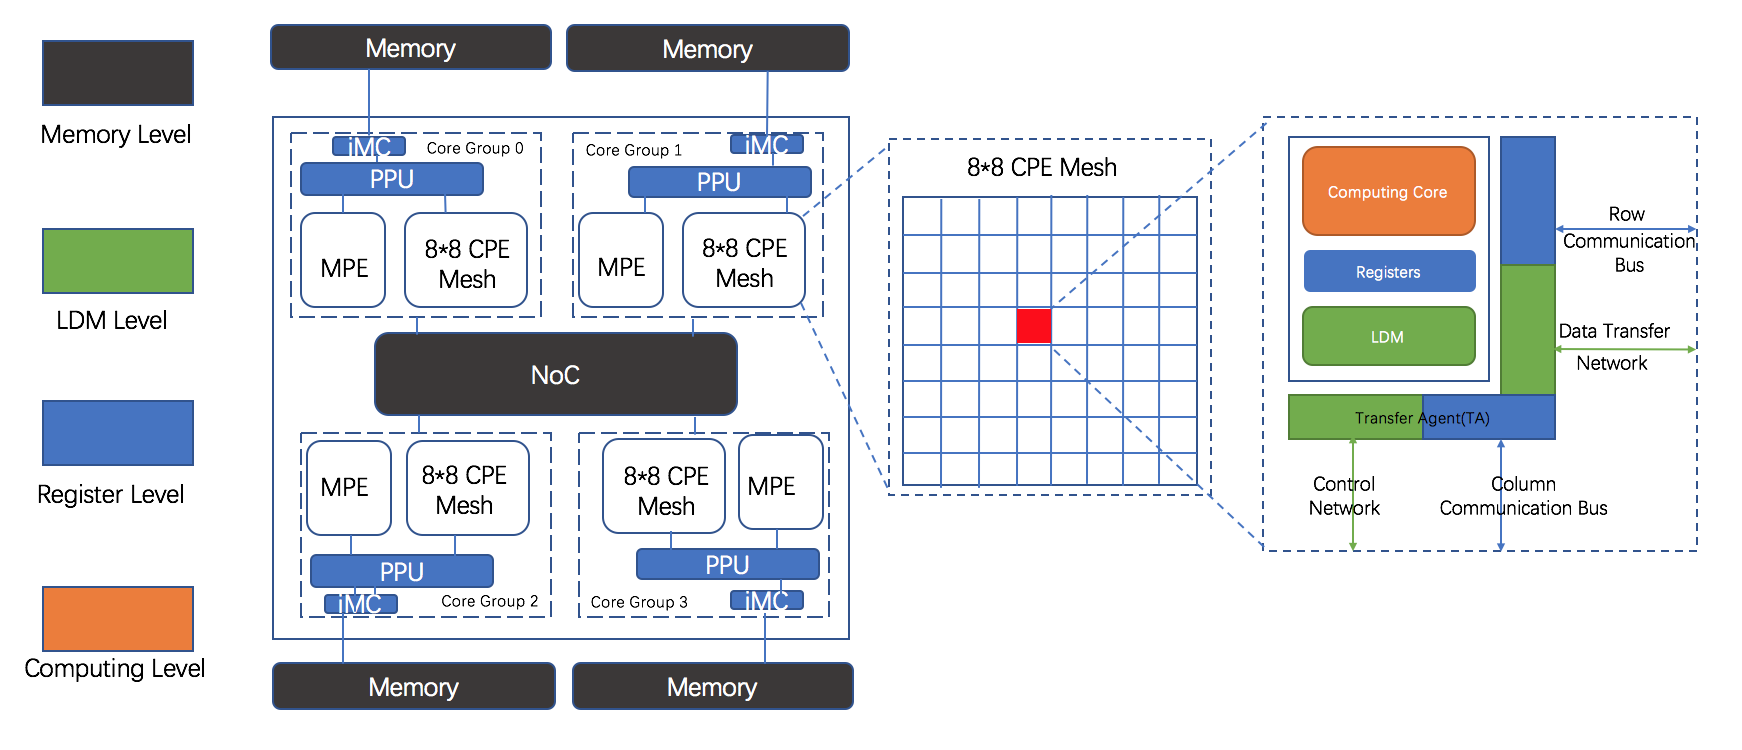
\includegraphics[scale=0.28]{Sunway.png}
\caption{The general architecture of the SW26010 many-core processor}
\label{figure:f1}
\end{figure} 



\subsection{Related Work}




In this section, we provide a formal description of the $k$-$means$ problem and then present the well-known approach, $Lloyd$ algorithm. Following is a discussion of the general parallel implementations and other supercomputer-based approaches.


\subsubsection{Problem Definition}
The purpose of the $k$-$means$ clustering algorithm is to find a group of clusters to minimize the mean distances between samples and their nearest centroids. Formalized, given $n$ samples {$\mathcal{X}^d$} = \{$x^d_i$\} $\in$ $\mathds{R}^d$, $i \in \{1\ldots n\}$, where each sample is a $d$-dimensional vector $x^d_i$ = ($x_{i1}$,\ldots, $x_{id}$) and we use $u$ to index the dimensions: $u \in \{ 1\ldots d \}$. We aim to find $k$ $d$-dimensional centroids {$\mathcal{C}^d$} = \{$c^d_j$\} $\in$ $\mathds{R}^d$, $j \in \{1 \ldots k\}$ to minimize the object $\mathcal{O}$($\mathcal{C}$):
$$  \mathcal{O}(\mathcal{C}) =    \frac{1}{n}\sum^{n}_{i=1} dis(x^d_i, c^d_{a(i)})   $$
Where $a(i)$ is the index of the nearest centroid for sample $x^d_i$:
$$ \ \ \ \ \ \ \ \ \ a(i)= arg\ min_{j\in \{1 \ldots k \} } dis({x^d_i}, c^d_j) $$
while $dis(x^d_i, c^d_j)$ is the $Euclidean$ distance between sample $x^d_i$ and centroid $c^d_j$:
$$ \ \ \ \ \ \ dis(x^d_i, c^d_j) = \sum^{d}_{u=1}(x_{iu}-c_{ju})^2 $$

\subsubsection{Lloyd Algorithm}
It is well-known that $k$-means problem is in NP-hard \cite{newling2016nested}. In the literature, several methods have been proposed to find efficient solutions \cite{newling2016fast,newling2016nested,ding2015yinyang,curtin2017dual,shen2017compressed,bottesch2016speeding}. While the most popular baseline is still the $Lloyd$ algorithm \cite{lloyd1982least}, which is composed by repeating the basic two steps below:
$$1.:\ a(i) = arg\ min_{j\in \{1 \ldots k \} }\ dis({x^d_i}, c^d_j)\ (Assign)$$
$$2.:\ c^d_j = \frac{\sum_{arg\ a(i)=j}x^d_i}{| arg\ a(i)=j |}\ \ \ \ (Update) $$
Note that those notations here are mainly from previous works by Hamerly \cite{hamerly2010making}, Newling and Fleuret \cite{newling2016fast}. We will apply customized notations only when needed. 
The first step above is to assign each sample into the nearest centroid according to the $Euclidean$ distance. The second step is to update the centroids by moving them to the mean of their assigned samples in the $d$-dimensional vector space. Those two steps are repeated until each $c^d_j$ is fixed. %The pseudo-code is shown in Algorithm 1.

%\documentclass[UTF8]{ctexart}

%\begin{algorithm}
%$$\mathcal{X}^d=\{x^d_i\}, i \in \{1\ldots n\}, clusters \ k \leq n$$
%\hspace*{0.02in} {\bf Initial:}
%$$random \ centroids \ {c^d_1} \ldots {c^d_j} \in R^d, j \in \{1\ldots k\}$$
%\hspace*{0.02in} {\bf repeat}

% \ \ \ \ \ Find nearest centroids:
%$$ \ \ \ \forall x^d \in \mathcal{X}^d: \ a(i)= arg\ min_{j\in \{1 \ldots k \} } dis({x^d_i}, c^d_j)$$
% \ \ \ \ \ Update centroids {$c_1$} \ldots {$c_j$}, j $\in$ \{1 \ldots k\}:
%$$ \forall j \in \{1 \ldots k\}: c^d_j \leftarrow \frac{\sum_{arg\ a(i)=j}x^d_i}{| arg\ a(i)=j |} $$ 
%\hspace*{0.02in} {\bf until} centroids stop changing
%
%\hspace*{0.02in} 
%{\bf Output:}$$ centroids \ {c_1} \ldots {c_j}, j\in \{1 \ldots k\}$$

%\end{algorithm}

\subsubsection{General Parallel $k$-$means$}

$k$-$means$ algorithm has been widely implemented in parallel architectures with shared and distributed memory using either SIMD or MIMD model targeting on multi-core processors \cite{dhillon2002data,hadian2014high,bohm2017multi}, GPU-based heterogeneous systems \cite{zechner2009accelerating,li2010speeding,torok2017k}, clusters of computer/cloud \cite{cui2014optimized,haut2017cloud}. 

In the parallel case, we use $l$ to index the processors (computing units) $\mathcal{P}$ and use $m$ to denote the total number of processors applied: $$\mathcal{P} = \{P_l\}, l \in \{1 \ldots m\}$$ The dataset $\mathcal{X}^d$ is partitioned uniformly into $m$ processors. Compared against the basic $Lloyd$ algorithm, each processor only assigns a subset ($\frac{n}{m}$) of samples from the original set $\mathcal{X}^d$ before  the $Assign$ step. Then the $Assign$ step is finished in parallel by $m$ processors. To formalize the steps, we obtain:
$$1.1: P_l \leftarrow {x^d_i}, i \in (1+(l-1)\frac{n}{m},l\frac{n}{m})  $$
$$1.2:\forall l \in (1,m), P_l:\ a(i) = arg\ min_{j\in \{1 \ldots k \} }\ dis({x^d_i}, c^d_j) $$ 

To facilitate communication between computing units, the Message Passing Interface (MPI) library is mostly applied in common multi-core processor environments. Performance nearly linearly increases with the limited number of processors as the communication cost between processes can be ignored in the non-scalable cases, as demonstrated in \cite{dhillon2002data}. Similarly, the $Update$ steps are finished by $m$ processors in parallel through MPI as well. Processors $P_l$ should communicate with each other before the final $c^d_j$ can be updated. CUDA is applied for implementing those communications when targeting on GPU-based systems \cite{zechner2009accelerating}, Hadoop is used in clusters \cite{cui2014optimized} and OpenStack for cloud architecture \cite{haut2017cloud}. We ignore the formal description of the general reduce-based parallel updating process here because it is not applicable to the proposed methods on our targeted hierarchical many-core processors. 

\subsubsection{Large-scale Parallel $k$-$means$ on Supercomputers}
%\footnote{Note that the cited supercomputer-based approaches either tested on their specific datasets \cite{kumar2011parallel,cai2015grouping} or published their a relative speedup rather than concrete execution time \cite{bender2015k}. It is not possible to compare concrete performance data from these sources with our approach. Instead, we compare actual execution time with other published results which do provide this data. Results of those experiments are shown in the final subsection in our experiment.}
In addition to general parallel $k$-$means$ implementations, other customized $k$-$means$ implementation targeting on supercomputers are more related to our work here. 

Kumar, et al \cite{kumar2011parallel} implemented the dataflow-partition based parallel $k$-$means$ on the $Jaguar$, a Cray XT5 supercomputer
%\footnote{This machine has been updated to $Titan$.} 
at Oak Ridge National Laboratory evaluated by real-world geographical datasets. Their implementation applys MPI protocols to achieve broadcasting and reducing and originally scaled the value of $k$ to more than 1,000s level.  

Cai, et al \cite{cai2015grouping} designed a similar parallel approach on $Gordon$, a Intel XEON E5 supercomputer at San Diego Supercomputer Center for grouping game players. They applied a parallel R function, $mclapply$, to achieve shared-memory parallelism and test different degree of parallelism by partitioning the original data-flow into different numbers of sets. They did not focus on testing the scalability of their approach but evaluated on the quality of the cluster. 

Bender, et al \cite{bender2015k} investigated a novel parallel implementation proposed for $Trinity$, the latest National Nuclear Security Administration supercomputer with Intel Knight's Landing processors and their $scratchpad$ two-level memory model. Their approach is the most state-of-the-art comparable work against our proposed methods which can not only partition dataflow, but also partition the number of target clusters $k$ by their $hierarchical$ two-level memory support - cache associated with each core and $scratchpad$ for share. Adapted originally from \cite{guha2003clustering}, their partitioning algorithm partitioned the input dataset into $\frac{nd}{M}$ sets, where $M$ is the size of the $scratchpad$, and then reduced $k\frac{nd}{M}$ centroids recursively if needed. Based on this partition, their approach scaled $d$ into 100,000s level.

A fundamental bottleneck in their approach is that  based on only two-level memory, it is still impossible to partition and then scale both $k$ and $d$ independently. This leads to the interaction constraint between $k$ and $d$ as discussed in their paper: 
$$ Z < kd < M$$
where $Z$ is the size of cache. This partition-based method is not efficient if all $k$ centroids could fit into one cache. In practice, this limits the value of $k$ to be less than 18 and $d$ to be greater than 152,917 in their experiments. We claim that our proposed approach with underlining data partitioning methods based on hierarchical many-core processors achieves the needed multi-level fully $nkd$ partition with architectural support to thoroughly solve this bottleneck. 

We formalize the background work of both general parallel $k$-$means$ and supercomputer-oriented implementations as shown in Table \ref{background}.

\subsubsection{Determining the optimal k}\label{background_J}
The number of culstering ($k$) need to be predetermined for typical $k$-$means$ algorithms. As claimed in the survey \cite{zhang2012review}, how to define this value is an critical question in the community, and inappropriate decision would yield poor quality of clustering results. 

Shi, et al. \cite{shi2004adaptive} proposed a basic method by gradually increasing the possible number of clusters and used the result when the distortion of solutions between current $k$ and $k$-1 is less than a static predefined threshold.
Chen, et al. \cite{chen2018improved} recently presented a method without any predefined threshold. It generates a formula by computing the difference between sum of distance inside and outside clusters.
%as following for our cases:
%$$ k = arg\ min_{k \in \{ 1 \dots n\}} \frac{1}{D(\mathcal{X}^d)} \sum_{j=1}^{k} D'(c_j^d,\mathcal{X}^d)  $$
%Where $D'(c_j^d,\mathcal{X}^d)$ denotes the sum of distances between samples clustered to centroid $c_j^d$ and samples in other clusters from the set $\mathcal{X}^d$. $D(\mathcal{X}^d)$ denotes the total sum of distances between samples in set $\mathcal{X}^d$. 
While this formulation didn't work in large-scale cases as it keeps monotonous increasing when the $k$ is greater than 2.

To solve this problem with a supercomputing-based approach, we introduce the notion of cluster radius $r(k)$ to $k$-$means$ clustering. To be specific, $r(k)$ is defined to be the smallest non-negative real number such that the sample set $\mathcal{X}^d$ can be covered by $k$ closed balls centered at sample points with radius $r(k)$. In other words,
\[
r(k) = \inf\{t: \exists x_{j_1}, \ldots, x_{j_k} \text{in } \mathcal{X}^d, \mathcal{X}^d\subseteq \bigcup_{1\leq s\leq k} B(x_{j_s}, t)\},
\]
where $B(x_{j_s}, t)$ stands for the Euclidean closed ball centered at $x_{j_s}$ with radius $t$. For instance, when $k = n$ the number of samples, we have $r(n) = 0$. It is easy to see that $r(k)$ is non-increasing with respect to $k$.

Radius has been widely used in clustering problems, such as approximating clustering~\cite{badoiu2002approximate} and incremental clustering~\cite{charikar2004incremental}, but not on $k$-$means$, because it is impossible to compute and measure all different radius values on large-scale datasets without help of modern supercomputer with efficient parallel processing techniques. The idea of determining the best $k$ is by measuring the rate of change of $r(k)$ with respect to $k$. If $r(k)$ does not shrink drastically as $k$ goes up by 1, we would regard this $k$ as a satisfying one. Rigorously speaking, let
\[
\Delta r(k) = r(k) - r(k+1).
\]
Then our optimal $k$ is taken as the integer minimizing this non-negative function $\Delta r$.

%We applied this state-of-the-art approach to determine the optimal $k$ value when clustering massive datasets without prior knowledge. 
%We will illustrate how we handle those steps efficiently in detail in the next section.
%In second step, the centroids are updated accordingly. It has been seen that performance increases nearly linearly with the number of processors. The multiple processors are communicated through MPI (the Message Passing Interface) library, which is a standardized, portable, and widely available message-passing system \cite{gropp1996high, snir1996mpi}. The communication cost between processes can be neglected nearly for large $m$. The algorithm is composed by repeating the four steps below:
%$$I.\ r_i \leftarrow {X^d_i} \ \ \ (i \in (1,m))$$
%$$II.\  for\ \ \  ({x^d_i} \in \mathcal{X}^d_{threadID} ) $$
%$$a(i) \leftarrow arg\ min_{j\in \{1 \ldots k \} }\ dis({x^d_i}, c^d_j) $$
%$$III.\ \ \ c^d_j \leftarrow \frac{\sum_{arg\ a(i)=j}x^d_i}{| arg\ a(i)=j |} $$
%$$IIII.\ \ \ \ \ \ \ \ \ \ \ \ \ \ \ R \leftarrow \sum^m_{j=1}{c^d_j}$$

\section{Multi-level large-scale $k$-$means$ design}
The scalability and performance of parallel $k$-$means$ algorithm on large-scale heterogeneous systems and supercomputers are mainly bounded by the memory and bandwidth. To achieve efficient large-scale $k$-$means$ on the Sunway supercomputer, we explore the hierarchical parallelism on our heterogeneous many-core architecture. We demonstrate the proposed scalable methods on three parallelism levels by how we partition the data. 

\begin{figure}
\centering
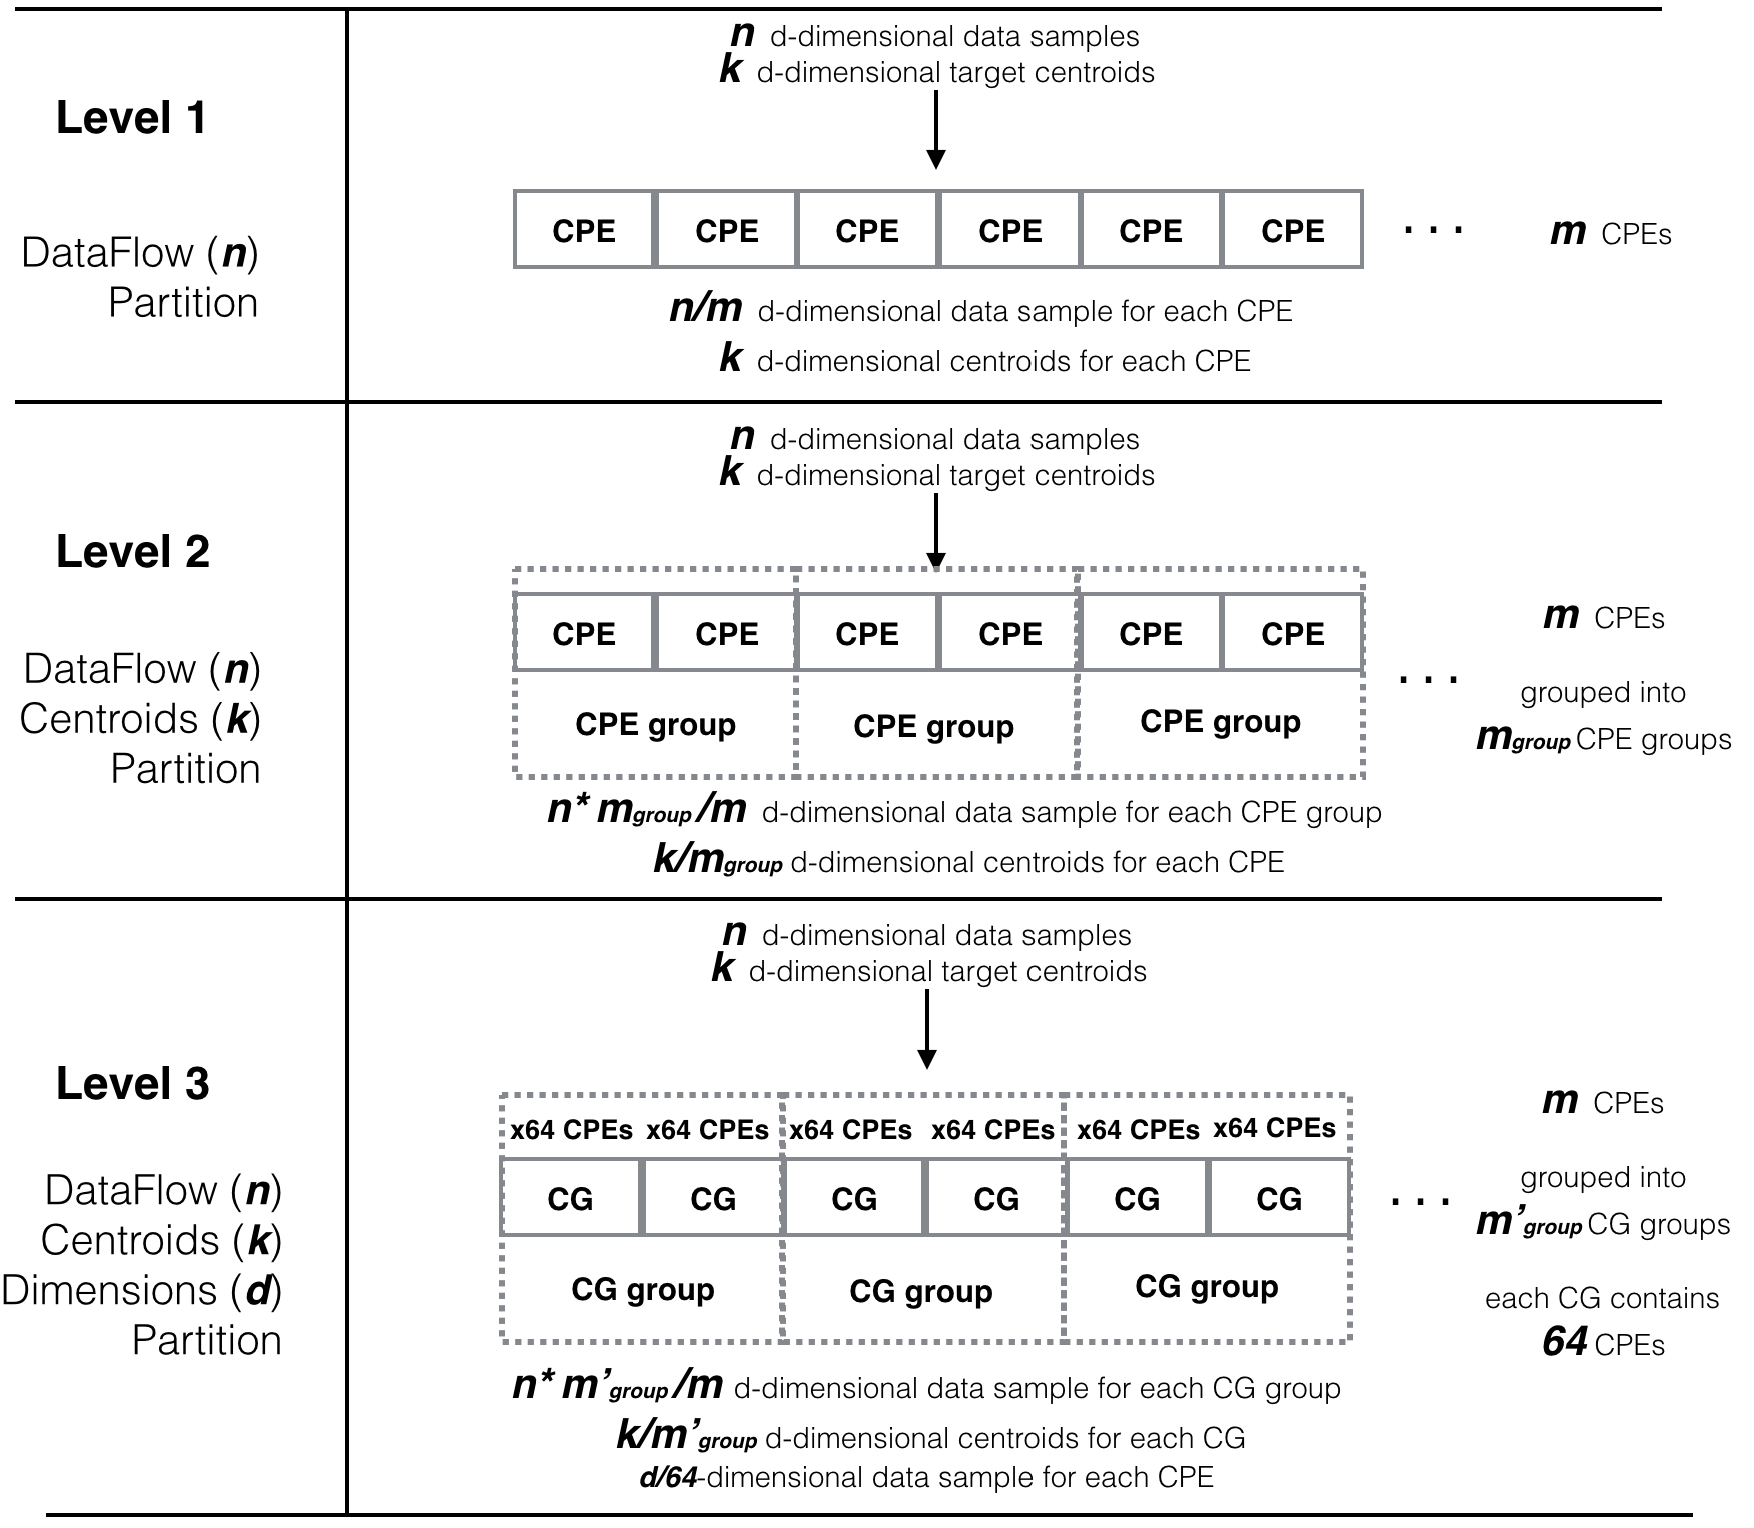
\includegraphics[scale=0.30]{partition.png}
\caption{Three-level $k$-$means$ design for data partition and parallelism on Sunway architecture}
\label{fig:fp}
\end{figure} 

%\begin{figure}
%\centering
%\includegraphics[scale=0.40]{ldm.png}
%\caption{The scalability of three-level parallel k-means on Sunway architecture}
%\label{fig:f2}
%\end{figure} 

\begin{itemize}

\item Level 1 - $DataFlow$ Partition: Store a whole sample and $k$ centroids on single-CPE 
\item Level 2 - $DataFlow$ and $Centroids$ Partition: Store a whole sample on single-CPE whilst $k$ centroids on multi-CPE
\item Level 3 - $DataFlow$,  $Centroids$ and $Dimensions$ Partition: Store a whole sample on multi-CPE whilst $k$ centroids on Multi-CG and $d$ dimensions on Multi-CPE

\end{itemize}

An abstract graph of how we partition the data into multiple levels is presented in Figure \ref{fig:fp}. 

\subsection{Level 1 - DataFlow Partition}

\begin{algorithm}
\caption{Basic Parallel $k$-$means$}
\label{alg:1}
\begin{algorithmic}[1]
\STATE \textbf{INPUT:} Input dataset $\mathcal{X} = \{x_i | x_i\in\mathds{R}^d, i\in[1, n]\}$, and initial centroid set $\mathcal{C} = \{c_j | c_j\in\mathds{R}^d, j\in[1,k]\}$
%\STATE \ //\emph{Setup Step:}
\STATE $P_l \xleftarrow{load} \mathcal{C},\ l \in \{1 \ldots m\}$ %//Each CPE loads the centroid set into LDM
\REPEAT
%\STATE // Fully-Parallel Process:
\STATE \ // Parallel execution on all CPEs:
\FOR {$l=1\  to\  m$}
\STATE Init a local centroids set $\mathcal{C}^{l} = \{c_j^l | c_j^l = \text{\textbf{0}}, j\in[1,k]\}$
\STATE Init a local counter $count^l = \{count_j^l | count_j^l = \text{0}, j\in[1,k]\}$
%\STATE \ //\emph{Assign Step:}
\FOR {$i = (1+(l-1)*\frac{n}{m})\ to\ (l*\frac{n}{m}) $}
\STATE $P_l \xleftarrow{load} x_i$ %//Load an input sample
\STATE $a(i) = arg\ min_{j \in \{1 \ldots k \} } dis(x_i, c_j)$
\STATE $c_{a(i)}^l = c_{a(i)}^l + x_i$
\STATE $count_{a(i)}^l =count_{a(i)}^l+1$
\ENDFOR
%\STATE \ //\emph{Update Step:}
\FOR {$j$ = $1$ $to$ $k$}
\STATE AllReduce $c_j^l$ and $count_j^l$
\STATE $c_j^l =  \frac{c_j^l}{count_j^l}$
\ENDFOR
\ENDFOR
\UNTIL{$ \mathcal{C}^{l} == \mathcal{C}\ $}
\STATE \textbf{OUTPUT:} $\mathcal{C}$
\end{algorithmic}
\end{algorithm}

In the simple case, we run the first step, $Assign$, on each CPE in parallel while using multi-CPE collaboration to implement the second step, $Update$. The pseudo code of this case is shown in Algorithm \ref{alg:1}.

The $Assign$ step is implemented similarly to the traditional parallel $k$-$means$ algorithm -- (1.1) and (1.2) as above. Given $n$ samples, we partition into multiple CPEs. Each CPE ($P_l$) firstly reads one sample $x_i$ and finds the minimum distances $dis$ from itself to all centroids $c_j$ to obtain $a(i)$.   
%To implement the $Update$ steps, 
Then two variables are accumulated for each cluster centroid $c_j$ according to $a(i)$, shown in line 11 and 12. The first variable stores the vector sum of all the samples assigned to $c_j$, notated as $c_{a(i)}^l$. The second variable counts the total number of samples assigned to $c_j$, notated as $count_{a(i)}^l$. 

In the $Update$ step, we first accumulate the $c_{j}^l$ and $count_{j}^l$ of all CPEs by performing two AllReduce operations, so that all CPEs can obtain the assignment results of the whole input dataset.  We use $register$ $communication$ \cite{fang2017swdnn} to implement intra-CG AllReduce operation and use MPI\_AllReduce for inter-CG AllReduce. After the accumulation, the $Update$ step is performed to calculate new centroids, as shown in line 15.
%\footnote{A detail description of this technique is provided in Appendix.} 

\subsubsection*{Analysis} 
Considering a one-CG task, we analyse the constraints on scalability in terms of memory limitation of each CPE. Based on the steps above, one CPE has to accommodate at least one sample $x_i$, all cluster centroids $\mathcal{C}$, $k$ centroids' accumulated vector sum $\mathcal{C}^{l}$ and $k$ centroids' counters $count^l$. Considering that each CPE has a limited size of LDM, we obtain the constraint ($\mathbf{C}_1$) below: 
$$\mathbf{C}_1:\ \ \ \ \ \ d(1+k+k)+k \leq LDM  $$
Since both the number of centroids $k$ and the dimension $d$ for each sample $x_i$ should at least be 1, we obtain two more boundary constraints ($\mathbf{C}_2$) and ($\mathbf{C}_3$) below, separately: 
$$\mathbf{C}_2:\ \ \ \ \ \ \ 3d+1 \leq LDM  $$
$$\mathbf{C}_3:\ \ \ \ \ \ \ 3k+1 \leq LDM  $$
%Assuming that one CPE can accommodate all the clusters and dimensions of the samples, so one CPE can complete the clustering calculation only once. The calculating results are sended to MPE for next calculation.
Now we analyse the performance under bandwidth bounds. Note that the $Assign$ step of computing $a(i)$ for each sample $x_i$ is completed fully in parallel on the $m$ CPEs. Given the bandwidth of multi-CPE architecture to be $B$, the DMA time of reading data from main memory can be simply formalized as: 
$$\mathbf{T}_{read}:\ \ \ (\frac{n*d}{m}+k*d)/B$$

Theoretically, a linear speedup for computing time to at most $n$ times against the serial implementation can be obtained for the $Assign$ step if we can apply $m = n$ CPEs in total.

The two AllReduce operations are the bottleneck process in the $Update$ step. The $register\ communication$ technique for internal multi-CPE communication guarantees a high-performance with a normally 3x to 4x speedup than other on-chip and Internet communication techniques (such as DMA and MPI) for this bottleneck process (referring to the experimental configuration section for detailed quantitative values). 
%note that the first two sub-steps (2.1) and (2.2) of computing partial vector sum and counter for $c^d_j$ are completed in parallel in each CPE without any data communication with other CPEs. The only bottleneck is (2.3) to update $c^d_j$ in which $m$ CPEs need to communicate to summarize the partial sum and counters they computed. The $register\ communication$ technique for internal multi-CPE communication guarantees a high-performance with a normally 3x to 4x speedup than other on-chip and internet communication techniques\footnote{Please refer to the experimental configuration section for detailed  quantitative values} . 
Given the bandwidth of $register\ communication$ to be $R$, the time for the AllReduce process can be formalized as:
$$\mathbf{T}_{comm}:\ \ \ \frac{n}{m}((1+k)*d)/R$$

\subsection{Level 2 - DataFlow and Centroids Partition}

\begin{algorithm}
\caption{Parallel $k$-$means$ for $k$-scale}
\label{alg:2}
\begin{algorithmic}[1]%[scale=0.2]
\STATE \textbf{INPUT:} Input dataset $\mathcal{X} = \{x_i | x_i\in\mathds{R}^d, i\in[1, n]\}$, and initial centroid set $\mathcal{C} = \{c_j | c_j\in\mathds{R}^d, j\in[1,k]\}$
%\STATE \ //\emph{Setup Step:}
\STATE $P_{l}\xleftarrow{load}{c_j}\,\ j \in (1+mod(\frac{l-1}{m_{group}})*\frac{k}{m_{group}},\ (mod(\frac{l-1}{m_{group}})+1)*\frac{k}{m_{group}})$
%\STATE $\{P\}_{l'} \leftarrow {x^d_i}, i \in (1+(l'-1)\frac{n*m_{group}}{m},\ l'\frac{n*m_{group}}{m})$
%\STATE $\{P\}_{l'} \xleftarrow{load} c_j,\ l' \in \{1 \ldots \frac{m}{m_{group}}\},\ j \in (1+ mod(\frac{l-1}{m_{group}})*\frac{k}{m_{group}} ,\ (mod(\frac{l-1}{m_{group}})+1)*\frac{k}{m_{group}})$ 
\REPEAT

\STATE \ // Parallel execution on each CPE group $\{P\}_{l'}$:
\FOR {$l'=1\  to\  \frac{m}{m_{group}}$}
\STATE Init a local centroids set $\mathcal{C}^{l'}$ and counter $count^{l'}$
%\STATE \ //\emph{Assign Step:}
\FOR {i = $(1+(l'-1)\frac{n*m_{group}}{m})$ $to$ $(l'\frac{n*m_{group}}{m})$ }
\STATE $\{P\}_{l'} \xleftarrow{load} x_i$ %//Load an input sample
\STATE $a(i)' = arg\ min_j\ dis(x_i, c_j)$
\STATE $a(i)  = min.\ a(i)'$
\STATE $c_{a(i)}^{l'} = c_{a(i)}^{l'} + x_i$
\STATE $count_{a(i)}^{l'} =count_{a(i)}^{l'}+1$
\ENDFOR
%\STATE \ //\emph{Update Step:}
\FOR {j =  $(1+ mod(\frac{l-1}{m_{group}})*\frac{k}{m_{group}})$ $to$ $((mod(\frac{l-1}{m_{group}})+1)*\frac{k}{m_{group}})$}
\STATE AllReduce $c_j^{l'}$ and $count_j^{l'}$
\STATE $c_j^{l'} =  \frac{c_j^{l'}}{count_j^{l'}}$
\ENDFOR
\ENDFOR
\UNTIL{$ \cup \ \mathcal{C}^{l'} == \mathcal{C}\ $}
\STATE \textbf{OUTPUT:} $\mathcal{C}$
\end{algorithmic}
\end{algorithm}

To scale the number of $k$ for cluster centroids $\mathcal{C}$, we use multiple (up to 64) CPEs in one CG to partition the set of centroids. The number of CPEs grouped to partition the centroids is denoted by $m_{group}$. For illustration, we use $l'$ to index the CPE groups \{P\}. Then we have:
$$ \{P\}_{l'} := \{P_l\},\ l \in (1+(l'-1)*m_{group}, l'*m_{group}) $$
The pseudo code of this case is shown in Algorithm \ref{alg:2}. To partition $k$ centroids on $m_{group}$ CPEs, we need to do a new sub-step against the previous case as shown in line 2.
%$$1.0:  P_{l} \leftarrow {c^d_j},$$ 
%$$j \in (1+ mod(\frac{l-1}{m_{group}})*\frac{k}{m_{group}} ,\ (mod(\frac{l-1}{m_{group}})+1)*\frac{k}{m_{group}}) $$
Then different from the $Assign$ step in above case, we partition each data sample $x_i$ in each CPE group as shown in line 8.
%$$1.1': \{P\}_{l'} \leftarrow {x^d_i}$$ $$i \in (1+(l'-1)\frac{n*m_{group}}{m},\ l'\frac{n*m_{group}}{m})  $$
After that, similar to (1.2), all $P_l$ in each $\{P\}_{l'}$ can still compute a partial value of $a(i)$ (named as $a(i)'$) fully in parallel without communication.   
%$$1.2':\forall l \in (1,\ldots,m), P_l:\ a(i)' = arg\ min_{j}\ dis({x^d_i}, c^d_j) $$
Note that the domain of $j$ in line 11 is only a subset of $(1,\ldots,k)$ as presented above in line 2, so we need to do one more step by data communication between CPEs in each CPE group to obtain the final a(i) as shown in line 10.
%$$1.3: \forall \{P\}_{l'}: a(i) = min.\ a(i)'$$

Then the $Update$ step is similar to previous case. We just view one CPE group as one basic computing unit, which conducts what a CPE did in the previous case. Each CPE only computes values of subset of centroids $\mathcal{C}$ and does not need further communications in this step as it only needs to store this subset.  

\subsubsection*{Analysis} 
To analyse the scalability of $k$ in this case, the amount of original $k$ centroids distributed in $m_{group}$ CPEs leads to a easier constraint of $k$ against the ($\mathbf{C}_3$) above: 
$$\mathbf{C'}_3:\ 3k+1 \leq m_{group}\ *LDM \ (m_{group} \leq 64) $$
%$$\mathbf{C}^`_3:\ 3k+1 \leq 64 *LDM  $$
Based on this, we can also easily scale the ($\mathbf{C}_1$) as follow: 
$$\mathbf{C'}_1:\ d(1+k+k)+k \leq m_{group}\ *LDM   \ (m_{group} \leq 64)$$
Note that we still need to accommodate at least one $d$-dimensional sample in one CPE, so the ($\mathbf{C}_2$) should be kept as before:
$ \mathbf{C'}_2:= \mathbf{C}_2$

As for performance, since $m_{group}$ CPEs in one group should read the same sample simultaneously, the processors need more time to read the input data samples than the first case, but only partial cluster centroids need to be read by each CPE:
$$\mathbf{T'}_{read}:\ \ \ (\frac{n*d*m_{group}}{m}+\frac{k}{m_{group}}*d)/B$$

As for the data communication needed, there is one more bottleneck process (line 12) than before. Comparing against the above cases, multiple CPE groups can be allocated in different processors. Those communication need to be done through MPI which is much slower than internal processor multi-CPEs $register$ $communication$. Given the bandwidth of network communication through MPI to be $M$, we obtain:
$$\mathbf{T'}_{comm}: \frac{k}{m_{group}}/R+\frac{n*m_{group}}{m}((1+k)*d))/M $$

\subsection{Level 3 - DataFlow and Centroids and Dimensions Partition}
\label{sec:level3partition}

\begin{algorithm}
\caption{Parallel $k$-$means$ for $k$-scale and $d$-scale}
\label{alg:3}
\begin{algorithmic}[1]
\STATE \textbf{INPUT:} Input dataset $\mathcal{X} = \{x_i | x_i\in\mathds{R}^d, i\in[1, n]\}$, and initial centroid set $\mathcal{C} = \{c_j | c_j\in\mathds{R}^d, j\in[1,k]\}$
\STATE $CG_{l''} \xleftarrow{load} c^d_j,\ l'' \in \{1 \ldots \frac{m}{64}\}, j \in (1+ mod(\frac{l''-1}{m'_{group}})*\frac{k}{m'_{group}} ,\ (mod(\frac{l''-1}{m'_{group}})+1)*\frac{k}{m'_{group}})$ 
%\STATE $P_{l} \leftarrow {x^u_i}, u \in (1+ mod(\frac{l-1}{64})*\frac{d}{64} ,\ (mod(\frac{l-1}{64})+1)*\frac{d}{64}) $
\REPEAT
%\STATE // Fully-Parallel Process:
\STATE \ // Parallel execution on each CG group $\{CG\}_{l''}$:
%\STATE $\forall l'' \in \{1 \ldots \frac{m}{64}\}, CG_{l''}\ in\ \textbf{parallel}:$
\FOR {${l''}=1\  to\  \frac{m}{64}$}
\STATE Init a local centroids set $\mathcal{C}^{l''}$ and counter $count^{l''}$
%\STATE \ //\emph{Assign Step:}
\FOR {i = $(1+(l''-1)\frac{n*m'_{group}}{m})$ $to$ $(l''\frac{n*m'_{group}}{m})$ }
\FOR {u = $(1+ mod(\frac{l-1}{64})*\frac{d}{64}$ $to$ $(mod(\frac{l-1}{64})+1)*\frac{d}{64})$}
\STATE $CG_{l''}$ $\leftarrow$ $x_i$ ($P_{l} \leftarrow {x^u_i}$)
\ENDFOR
%\STATE $\{P\}_{l'} \xleftarrow{load} x_i$ %//Load an input sample
\STATE $a(i)' = arg\ min_j\ dis(x_i, c_j)$
\STATE $a(i)  = min.\ a(i)'$
\STATE $c_{a(i)}^{l''} = c_{a(i)}^{l''} + x_i$
\STATE $count_{a(i)}^{l''} =count_{a(i)}^{l''}+1$
\ENDFOR
%\STATE \ //\emph{Update Step:}
\FOR {j =  $(1+ mod(\frac{l''-1}{m'_{group}})*\frac{k}{m'_{group}})$ $to$ $((mod(\frac{l''-1}{m'_{group}})+1)*\frac{k}{m'_{group}})$}
\STATE AllReduce $c_j^{l''}$ and $count_j^{l''}$
\STATE $c_j^{l''} =  \frac{c_j^{l''}}{count_j^{l''}}$
\ENDFOR
\ENDFOR
\UNTIL{$ \cup \ \mathcal{C}^{l''} == \mathcal{C}\ $}
\STATE \textbf{OUTPUT:} $\mathcal{C}$
\end{algorithmic}
\end{algorithm}

To scale the number of dimension $d$ for each sample $x_i$ and further scale $k$, we store and partition one $d$-dimensional sample by one CG with 64 CPEs and then implement the algorithm on multiple CGs.  The pseudo code of this case is shown in Algorithm \ref{alg:3}.

Recall we use $u$ to index the data dimension: $u \in (1\ldots d)$; Now we use $l''$ to index the CGs and $m'_{group}$ to denote the number of CGs grouped together to partition $k$ centroids. Consider that  we apply $m$ CPEs in total and each CG contains 64 CPEs, then we have $l'' \in (1, \ldots,\frac{m}{64})$, $m'_{group} \leq \frac{m}{64}$ and:
$$CG_{l''} := \{P_l\},\ l \in (1+64(l''-1),\ 64l'') $$
To partition $k$ centroids on multiple CGs, we obtain an updated step against the previous case as shown in line 2.
%$$1.0': CG_{l''} \leftarrow {c^d_j},$$ 
%$$j \in (1+ mod(\frac{l''-1}{m'_{group}})*\frac{k}{m'_{group}} ,\ (mod(\frac{l''-1}{m'_{group}})+1)*\frac{k}{m'_{group}}) $$
To partition each $d$-dimensional sample $x^d_i$ on 64 CPEs in one CG, we obtain the following step as shown in line 9.
%$$1.1'':  P_{l} \leftarrow {x^u_i},$$ 
%$$u \in (1+ mod(\frac{l-1}{64})*\frac{d}{64} ,\ (mod(\frac{l-1}{64})+1)*\frac{d}{64}) $$

Similar to the above case, all $CG_{l''}$ in each CG group compute the partial value $a(i)'$ fully in parallel and then communicate to obtain the final $a(i)$.
%$$1.2'':\forall l'' \in (1,\ldots,\frac{m}{64}), CG_{l''}:\ a(i)' = arg\ min_{j}\ dis({x^d_i}, c^d_j) $$
%$$1.3': \forall \{CG\}: a(i) = min.\ a(i)'$$
Multi-CG communication in multiple many-core processors (nodes) is implemented through MPI interface. Then the $Update$ step is also similar to the previous case. Now we view one CG as one basic computing unit which conducts what one CPE did before and we view what a CG group does as what a CPE group did before.

\subsubsection*{Analysis} 
In this case, each CG with 64 CPEs accommodates one $d$-dimensional sample $x_i$. Then we can scale the previous ($\mathbf{C}_2$) as follow:
$$\mathbf{C''}_2:\ 3d+1 \leq 64 *LDM  $$
Consider we use totally $m'_{group}$ CGs to accommodate $k$ centroids in this case, then ($\mathbf{C}_3$) will scale as follow: 
$$\mathbf{C''}_3:\ 3k+1 \leq {m'}_{group} *64*LDM  $$
Note that the domain of $m'_{group}$ seems limited by the total number of CPEs applied, $m$. But in fact, this number can be large-scale as we target on the supercomputer with tens of millions of cores. Finally, ($\mathbf{C}_1$) will scale as follow:
$$\mathbf{C''}_1:\ d(1+k+k)+k \leq 64*m'_{group}*LDM  $$
which is equal to:
$$\mathbf{C''}_1:\ d(1+k+k)+k \leq m*LDM  $$
$\mathbf{C''}_1$ is the breakthrough contribution over other state-of-the-art work \cite{bender2015k}: the total amount of $d*k$ is not limited by a single or shared memory size any more. It is fully scalable by the total number of processors applied ($m$). In a modern supercomputer, this value can be large-scaled up-to tens of millions when needed.  

Considering performance, note that $m'_{group}$ CGs (64 CPEs in each) in one group should read the same sample simultaneously. In another aspect, each CPE only needs to read a partial of the given $d$-dimension of original data sample together with  a partial of $k$ centroids similarly as before, then we obtain a similar reading time:  
%$$\mathbf{T''}_{read}:\ \ \ (\frac{n*d*m'_{group}}{m}+\frac{k}{m'_{group}}*\frac{d}{64})/B$$
\begin{equation}
  \label{eq:tread}
  $$\mathbf{T''}_{read}:\ \ \ (\frac{n*d*m'_{group}}{m}+\frac{k}{m'_{group}}*\frac{d}{64})/B
\end{equation}


Comparing against the above cases, multiple CGs in CG groups allocated in different many-core processors need communication to update centroids through MPI. Given the bandwidth of network communication through MPI to be $M$, the cost between multiple CG groups can be formalized as:
%$$\mathbf{T''}_{comm}: (\frac{k}{m'_{group}}+\frac{n*m'_{group}}{m}((1+k)*d))/M $$
\begin{equation}
  \label{eq:tcomm}
  \mathbf{T''}_{read}:\ \ \ (\frac{n*d*m'_{group}}{m}+\frac{k}{m'_{group}}*\frac{d}{64})/B
\end{equation}

The network architecture of Sunway TaihuLight is a two-level fat tree. 256 computing nodes are connected via a customized inter-connection board, forming a \emph{super-node}. All super-nodes are connected with a central routing server. The intra super-node communication is more efficient than the inter super-node communication. Therefore, in order to improve the overall communication efficiency of our design, we should make a CG group located within a super-node if possible. 

%Furthermore, for cases where we cannot avoid inter super-node communication, we call a customized MPI library, which is optimized targeting the network architecture based on an intra super-node communication first strategy.

\subsection{Impact of Multi-level Large-scale Design}
As described in the background section,  \textit{Level 1} is based on the well-researched parallel $k$-$means$ deign using dataflow partition ($n$-partition) which has been implemented on other supercomputers including $Jaguar$ \cite{kumar2011parallel} and $Gordon$ \cite{cai2015grouping} to process regular big dataset with up to 1,000s centroids and small number of dimensions. \textit{Level 2} provides similar functionality to Bender et al. \cite{bender2015k} approach targeting on $Trinity$, implementing both dataflow and centroids partition ($n$$k$-partition) to successfully handle big dataset with large-scale dimensions. \textit{Level 3} is our original first ever approach to finally achieve all dataflow, centroids and data samples ($n$$k$$d$-partition) simultaneously to successfully handle big dataset with both large-scale dimensions and large-scale centroids achieving high performance.  

The multi-level large-scale approaches together also give us the needed flexibility to handle both high dimensional and low dimensional dataset efficiently on supercomputer, which also breaks the limitation in current state-of-the-art design by Bender et al. \cite{bender2015k} which claims only efficient for dataset with larger than 100,000 dimensions. 

\section{Auto-clustering Layer Design and Implementation}\label{auto-implementation}

In Section~\ref{background_J}, we described a method to determine the optimal number of centroids ($k$) for the $k$-means algorithm on a given input set. This method is very useful in limited-resources settings, where we cannot run multiple instances of the $k$-means algorithm (for different $k$), but instead we need to determine the value of $k$ upfront. However, the method is still computationally expensive and, in the supercomputer settings, we have enough resources to run $n$ instances of $k$-means algorithm in parallel (for $k \in \{1,2,\dots,n\}$. We can then use a function similar to the one proposed in Section~\ref{background_J} for calculating radius $r(k)$ as an evaluation function to estimate the quality of solution that each instance of the $k$-means algorithm derives. This leaves us with two practical problems - how to automatically select the data partitioning method to process the workload when the value of $k$ changes and how to allocate resources of a supercomputer fo different instances of the $k$-means algorithm.
%To efficiently process massive data without prior knowledge, we need an auto-learning layer to determine the optimal value of targeting centroids ($k$). Instead of predicting the optimal value before execution under limited computing resources, our supercomputing based large-scale approach can process all possible $k$ values in parallel within a reasonable time and then determine the actual optimal value by our evaluation function. In detail, we design and implement: 
\subsection{Self-aware Auto Dataflow Partition} 
A self-aware method to auto partition dataflow into 3 levels based on the targeting $k$ values. This method is mainly guided by the scalability of each level of data partitioning. Based on the limitations presented in formulations ($\mathbf{C}_1,\mathbf{C'}_1,\mathbf{C''}_1$) above, we can easy compute the range of possible $k$ values for each level: $k \leq \frac{LDM-d}{1+2d}$ for level-1, $k \leq \frac{64LDM-d}{1+2d}$ for level-2 and $k \leq \frac{m*LDM-d}{1+2d}$ for level-3. By concatenating the ranges, we obtain the self-aware 3-stage roofline model to guide the data partitioning as shown in figure~\ref{roofline}.

\subsection{Fairness Resource Allocation and Task Scheduler}
Dividing the resources of the supercomputer between the $n-1$
instances of the $k$-means algorithm can be looked at as a scheduling
problem, where we need to schedule $n-1$ heterogeneous tasks on a
given set of resources. The tasks are heterogeneous because, for
different $k$, $k$-means algorithm will do different partitioning of
the data (see the previous section), different degree of parallelism
(more parallelism for larger values of $k$) and different
computational costs. Therefore, dividing the resources optimally
between the instances of the algorithm will be suboptimal.
Furthermore, it is not possible to statically
compute the precise cost of executing one instance of the algorithm on
a given set of resources because, in addition to the reading (equation
\ref{eq:tread}) and communication (equation \ref{eq:tcomm}) time that
can easily be estimated, there is also a computation time that depends
on the number of iteration for a particular value of $k$ and a
particular input, and this number cannot be computed
statically. Therefore, we need to use some heuristics for resource
allocation.

The approach we take in this paper is to use a cost function,
$T''(k,m,m'_{group})$, as an estimation of the cost of executing an
instance of $k$-means on $m$ CPEs and $m'_{group}$ CPE groups for each
centroid. The scheduling problem can then be seen as the optimisation
problem of finding the minimum of the function

$$A(m_1,\dots,m_{n-1}, m_1', \dots
m_{n-1}') = \sum_{i=1}^{n-1} T''(i,m_i,m_i')$$

\noindent
with the following constraints: $1 \leq m_i \leq p \; (\mbox{for } i \in
\{1,\dots,n-1\}), \sum_{i=1}^{n-1} m_i \leq p, 0 \leq m_i' \leq
\frac{p}{q} \; (\mbox{for } i \in
\{1,\dots,n-1\}), \sum_{i=1}^{n-1} m_i' = \frac{p}{q},$
where $p$ is the total number of CPEs and $q$ is the number of CPEs
per group ($64$ in our case). We use $T''(k,m,m')=T''_{read}(k,m,m')+T''_{comm}(k,m,m')$ as a 
cost function, where $T''_{read}$ and $T''_{comm}$ are given in the equations
\ref{eq:tread} and \ref{eq:tcomm}. Note that there will be additional
constraints on the values that $m'$ can take, which will depend on
$k$, $m$ and also the level of data partitioning.

The algorithm that we use to solve the posed optimisation problem is
given in Algorithm~\ref{alg:resourceAllocAlg}, which is based on a
greedy approach. We initially allocate one CPE and zero CPE groups to each of the $n-1$ instances
of the $k$-means algorithm (lines 2--4). Then, in successive
iterations, we add one more CPE to the instance which has the highest
cost (therefore reducing its cost), until all of the CPEs are
allocated (lines 6--9). This, effectivelly, gives us
the assignment of $m_1,m_2,\dots,m_{n-1}$. We repeat the similar
procedure to assign $m'_1,\dots,m_{n-1}'$ (lines 12--19).
However, as noted above, we must take into account the
constrants for the value of $m'$ when trying to increase it. For this
purpose, we use the set $S$ to track downthe instances for which it
is possible to improve the cost by adding more CPE groups. This set
initially contains all instances (line 11), but when we discover that
for some instance it is not impossible to increase $m'$ or that
increasing it does not yield improvement in cost, we eliminate it from
$S$ (line 17). 

\begin{algorithm}
\caption{Resource Allocation Algorithm}
\label{alg:resourceAllocAlg}
\begin{algorithmic}[1]
  \STATE \textbf{INPUT:} Cost function $T''(k,m,m')$, number of CPEs
  $p$, number of CPEs per group $q$, number of points $n$
  \FOR {i=$1$ to $n-1$}
  \STATE $m_i = 1$; $m'_i= 0$
  \ENDFOR
  \STATE remProc = $p - (n-1)$
  \WHILE {remProc $>0$}
  \STATE $i = \mbox{argmin}_{j=1}^{n-1} T''(j,m_j,m'_j)$
  \STATE $m_i = m_i + 1$; remProc $=$ remProc $-1$
  \ENDWHILE
  \STATE remGroups = $\frac{p}{q}$
  \STATE  $S = \{1,\dots,n-1\}$
  \WHILE {(remGroups $>0$ and $|S|>0$)}
  \STATE $i= \mbox{argmin}_{j=1, j \in S}^{n-1} T''(j,m_j,m'_j)$
  \IF {$m'_i$ can be increased and $T''(i,m_i,m'_i)$ would be
    decreased by that}
  \STATE $m'_i = m'_i+1$; remGroups $=$ remGroups $-1$
  \ELSE
  \STATE $S = S \setminus \{i\}$
  \ENDIF
  \ENDWHILE
  \STATE \textbf{OUTPUT:} $\{m_1,\dots,m_{n-1},m'_1, \dots, m'_{n-1}\}$
\end{algorithmic}
\end{algorithm}




%Since our aim is to execute, at the same time, $n-1$ instances of the $k$-means algorithm,
%for each $k$ between $1$ and $n-1$, we need to find a way to divide
%the resources of the supercomputer to efficiently execute all of these
%computations. Different instances of the algorithm will have different
%partitioning of the data (see Section~\ref{auto-implementation}),
%different degrees of parallelism (more parallelism for larger values
%of $k$) and different computational cost. Therefore, the problem of
%allocating resources for these instances can be seen as for . In Section~\ref{sec:level3partition}, we showed the costs of reading (equation \ref{eq:tread}), communication (equation \ref{eq:tcomm}) and computation (equation \ref{eq:tcomp}) for a single instance of the $k$-means algorithm with 3-level partitioning of data. We can see that these costs depend on the value of $k$ (the number of clusters), $m$ (the number of allocated CPEs) and $m'_{group}$ (the number of CGs grouped together to partition the $k$ centroids). Therefore, if we estimate a total cost of one instance of the $k$-means algorithm as $T''=T''_{read}+T''_{comm}+T''_{comp}$, then $T''$ can be seen, for a fixed $k$,  as a function of $m$ and $m'_{group}$ ($T''=T''_k(m,m'_{group}))$. If we denote by $m_k$ and $m_k'_{group}$ the nubmer CPEs and the number of CGs grouped together to the $k$-means instance with fixed $k$, then the problem of allocating resources for all instances of the $k$-means problem, for $k\in\{1,2,\dots,n\}$ can be posed as a linear programming problem of choosing ($\{m_1,m_2,\dots,m_{n-1}\}$), with $m_i \in \{1,2,\dots,M\}$ and $\sum_{i=1}^{n-1}m_i \leq M$ ($M$ being a total number of CPEs) and $\{m_1'_{group}, m_2'_{group}, \dots, m_{n-1}'_{group}\}$ such that

%$$\sum_{i=1}^{n-1} T''_i(m_i,m_i'_{group})$$

%achieves minimum.



%A fairness resource allocation method to run the heterogeneous workflows on the many-core supercomputer in parallel and keep load balancing. This method is mainly guided by the difference from performance of each data partitioning level. Instead of an easy roofline model as above based on the boundary of scalability, the performance difference coming from pipeline reading, communication and computation time with non-deterministic number of iterations  can not be easily formulated. 
    
%To achieve efficient resource allocation, we apply empirical approach to determine the number of reserved processors (from only several CPEs in one core group to even multiple distributed nodes) for each task. We launch tasks to processors proportional to their targeting number of centroids ($k$) to keep load balancing. For example, a group of processors will only launch one task if its $k = \frac{n}{2}$, while tasks with $k = n-1$ and $k=2$ will be launched to another group of processors.

\subsection{Evaluation Function}
A correct evaluation function to determine the optimal $k$.


%(1) A self-aware method to auto partition dataflow into 3 levels based on the targeting $k$ values; (2) A fairness resource allocation method to run the heterogeneous workflows on the many-core supercomputer in parallel and keep load balancing; (3) A correct evaluation function to determine the optimal $k$.  

\begin{figure}
\centering
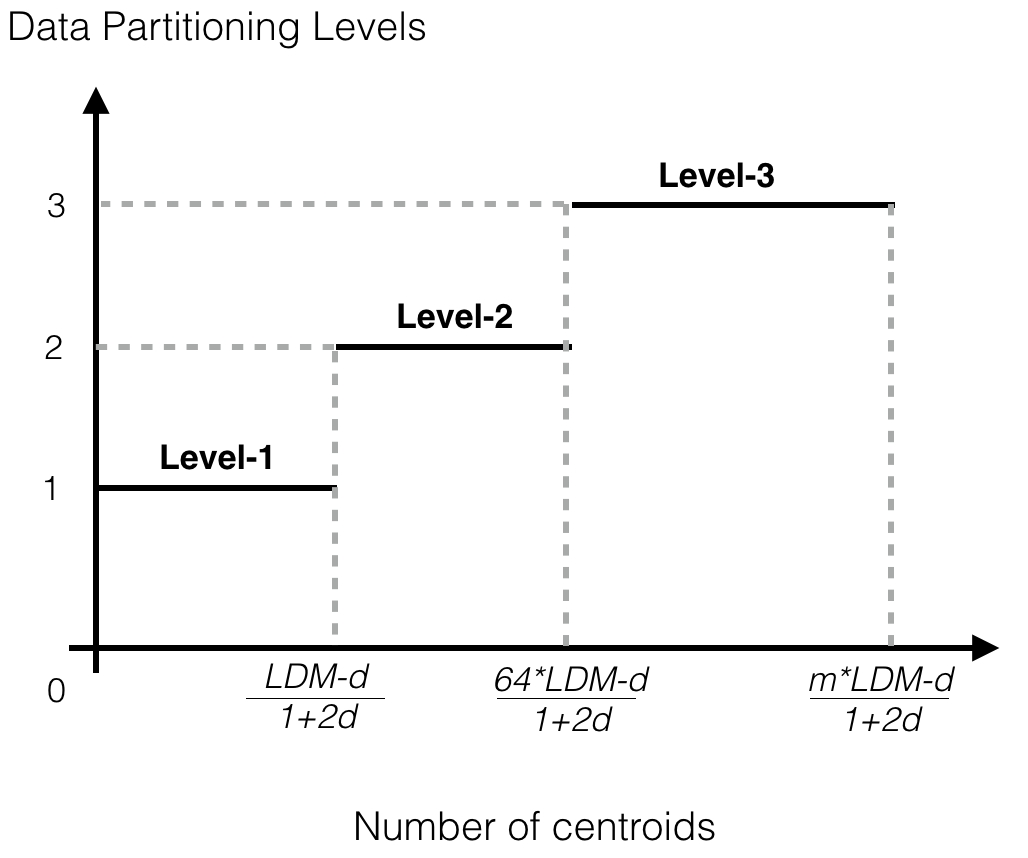
\includegraphics[scale=0.45]{roofline.png}
\caption{Self-aware Roofline Model for Auto Data Partitioning}
\label{roofline}
\end{figure}

%\subsection{Self-aware Data Partitioning}
%\subsection{Fairness Resource Allocation}
%\subsection{Evaluation Function}

%To auto-determine the optimal $k$ value for massive data without prior knowledge, we implement the evaluation function on the many-core processors in parallel.

\section{Experimental Evaluation}
We describe our experimental evaluation in this section. We run our proposed methods on Sunway TaihuLight, with a hierarchical SW26010 many-core processor as the main processor. architecture. 

%This section is structured as follows: 
We first describe the datasets applied and then discuss the experimental metrics. The experimental strategy is presented followed by the results on the three scalable levels, a comparison between partitioning strategies, and analysis. 


\subsection{Experimental Datasets}
The datasets we applied in experiments come from well-known benchmark suites including UCI Machine Learning Repository\cite{uci} and ImgNet \cite{imgnet}. We briefly present the datasets in Table \ref{t1}, where the first three normal size benchmarks ({\it Kegg Network, Road Network, US Census 1990}) are from UCI and the final high-dimensional benchmarks ({\it ILSVRC2012}) are from ImgNet.

We do not describe the more detailed technical and background descriptions of those benchmarks as they are well-known and commonly applied in the literature. 

\begin{table}
  \caption{Benchmarks from UCI and ImgNet}
  \label{t1}
   \begin{tabular}{p{2.5cm} p{1.5cm} p{1.5cm}p{1.5cm} c c c c}
 % \begin{tabular}{l c c c c}
      \hline
    Data Set &n & k & d\\
       \hline
    %Gassensor &1.4E4 &256 &129 \\
    Kegg Network &6.5E4 &256 &28  \\
    Road Network &4.3E5 &10,000 &4 \\
    US Census 1990 &2.5E6 &10,000 &68 \\
    \hline
    ILSVRC2012 (ImgNet) &1.3E6 &160,000 &196,608 \\
%    ILSVRC2012 &8.1E6 &1000 &4096 \\
%    RCV1 &1.9E5 &103 &1979  \\
    \hline
  \end{tabular}
\end{table}


\subsection{Experimental Design and Metrics}
The experiments have been conducted to demonstrate scalability, high performance and flexibility by increasing the number of  centroids $k$ and number of dimensions $d$ on multiple benchmarks with vary data size $n$. The three-level designs are tested targeting different benchmarks.  
Different hardware setup will be provided for testing different scalable levels:
\begin{itemize}
\item{\it Level 1 - } One SW26010 many-core processor is applied, which contains 256 64-bit RISC CPEs running at 1.45 GHz, grouped in 4 CGs in total. As 64 KB LDM buffer is associated with each CPE and 32 GB DDR3 memory is shared for the 4 CGs, we setup 16 MB LDM and 32 GB DDR3 memory support in total. The theoretical memory bandwidth for register communication is 46.4 GB/s and for DMA is 32 GB/s.
\item{\it Level 2 - } Up-to 256 SW26010 many-core processors are applied, which contains 65,536 64-bit RISC CPEs running at 1.45 GHz, grouped in 1,024 CGs in total. We setup 4 GB LDM and 8 TB DDR3 memory support in total. The theoretical memory bandwidth for register communication is 46.4 GB/s and for DMA is 32 GB/s. The bidirectional peak bandwidth of the network between multiple processors is 16 GB/s.
\item{\it Level 3 - } Up-to 4,096 SW26010 many-core processors are applied, which contains 1,064,496 64-bit RISC cores running at 1.45 GHz, grouped in 16,384 CGs in total. In this setup,  64 GB LDM and 128 TB DDR3 memory  are supported in total. The bidirectional peak bandwidth of the network between multiple processors is 16 GB/s.
\end{itemize}
The main performance metric we are concerned with here is {\it one iteration completion time}. Note that the total number of iterations needed and the quality of the solution (precision) are not considered in our experiments as our work does not relate to the optimization of the underlining Lloyd algorithm or the solution of $k$-$means$ algorithm. 

\subsection{Experimental Results and Analysis}
\label{results}
\begin{figure}
\centering
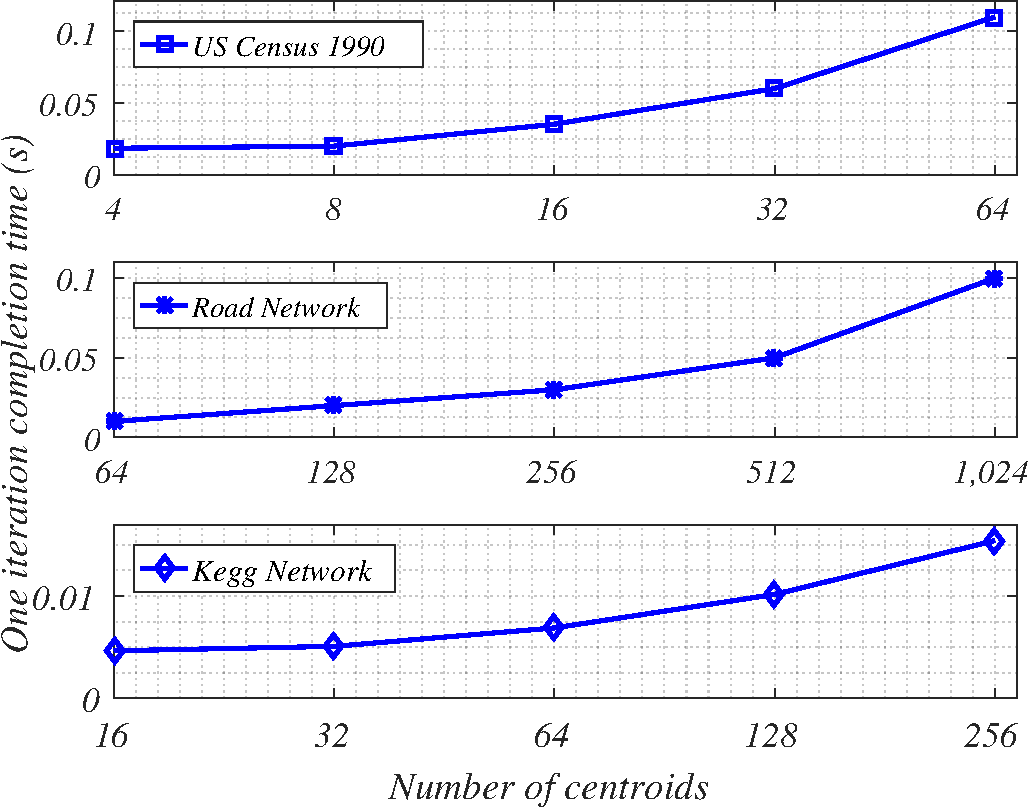
\includegraphics[scale=0.40]{level-1.pdf}
\caption{Level 1 - dataflow partition}
\label{level1}
\end{figure} 

\begin{figure}
\centering
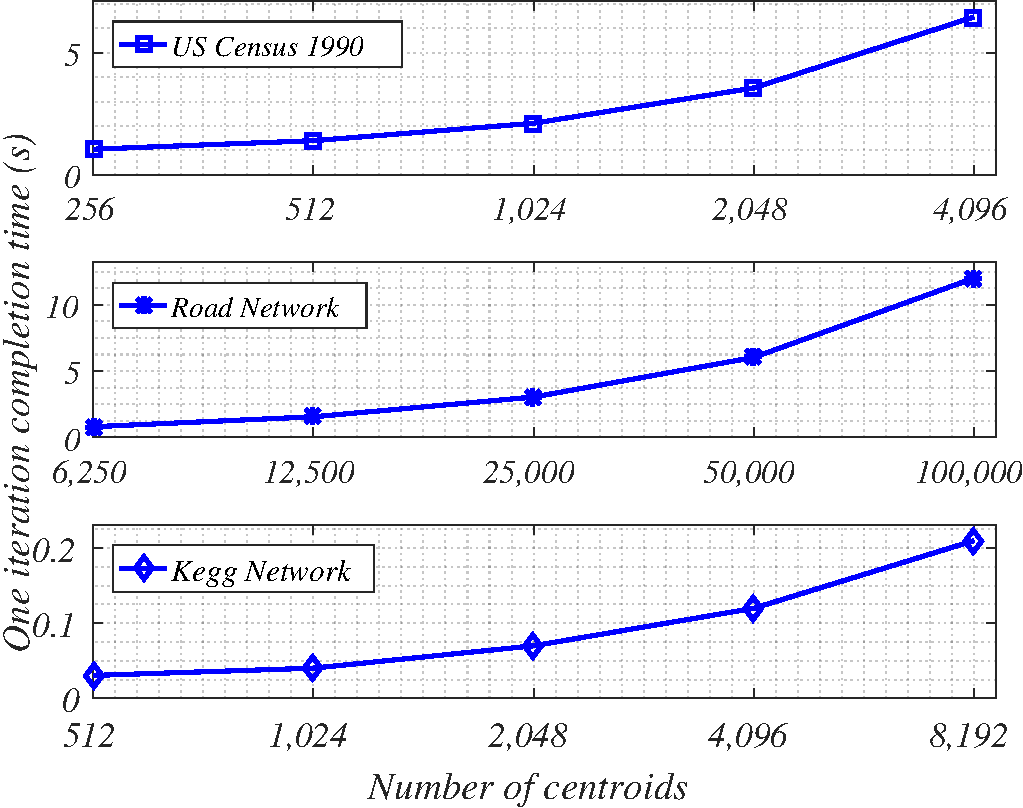
\includegraphics[scale=0.45]{level-2.pdf}
\caption{Level 2 - dataflow and centroids partition}
\label{level2}
\end{figure}

We report the results of three different partition strategies: \textit{Level 1} -- a baseline single-level partition strategy, \textit{Level 2} -- an implementation of a state-of-the-art two-level partition strategy used in recent supercomputer implementations\cite{bender2015k}, and \textit{Level 3} -- our novel three-level partition strategy.

Since each partitioning strategy is only able to run successfully at certain ranges of $k$ and $d$, it is not possible to compare them directly across the whole range benchmarks as the benchmarks have limits in terms of dataset size. For this reason, we first evaluate each strategy independently on the most suitable benchmarks for the strategy in question to show how each performs in the range for which they are most suited. The second part of our evaluation compares the partition strategies directly on benchmarks where the possible range of $k$ and $d$ overlap. This shows how our proposed \textit{Level 3} strategy scales significantly better than \textit{Level 2} over varying $k$, $d$, and number of computational nodes.

\subsubsection{Level 1 - dataflow partition}
The \textit{Level 1} ($n$-partition) parallel design is applied to three UCI datasets ({\it US Census 1990, Road Network, Kegg Network}) with their original sizes ($n$ = 2,458,285, 434,874 and 65,554 separately) and data dimensions ($d$ = 68, 4 and 28) for cross number of target centroids ($k$). The purpose of these experiments is to demonstrate the efficiency and flexibility of this approach on datasets with relatively low size, dimensions and centroid values. Figure \ref{level1} shows the {\it one iteration completion time} for those datasets over increasing number of clusters, $k$. 
As the number of $k$ increases, the completion time on this approach grows linearly.
%As the number of $k$ increases, the completion time from our approach always keep in a low level with a super linear speedup. 
%For example, as shown in the Figure \ref{level1}, we can finish one iteration within 0.1 seconds for 2,458,285 {\it US Census 1990} data samples with 64 centroids and 68 dimensions which demonstrate our claimed efficiency and flexibility.  


\subsubsection{Level 2 - dataflow and centroids partition}
The level 2 ($nk$-partition) parallel design is applied to same three UCI datasets as above, but for a large range of target centroids ($k$). The purpose of these experiments is to demonstrate the efficiency and flexibility of the proposed approaches on datasets with  large-scale target centroids (less than 100,000). Figure \ref{level2} shows the {\it one iteration completion time} of the three datasets of increasing number of clusters, $k$. As the number of $k$  increasing, the completion time from this approach grows linearly. We conclude that this approach works well when one dimension is varied up to the limits previously published. 

%For example, as shown in the Figure \ref{level2}, we can finish one iteration within 13 seconds for 434,874 {\it Road Network} data samples with 100,000 centroids and 3 dimensions which demonstrate our claimed high performance, scalability and flexibility.  ImgNet benchmark is also applied to test this level design for comparing against the level3 design, which we will analyse in detail later.

\begin{figure}
\centering
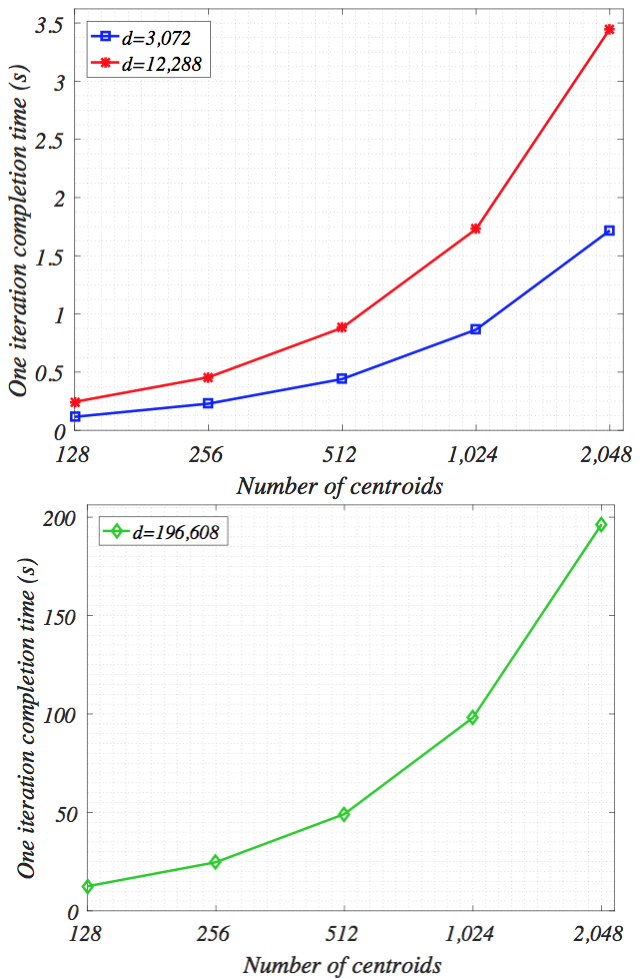
\includegraphics[scale=0.50]{level-3.png}
\caption{Level 3 - dataflow, centroids and data-sample partition}
\label{level3}
\end{figure}



\subsubsection{Level 3 - dataflow, centroids and dimensions partition}
The \textit{Level 3} ($nkd$-partition) parallel design is applied to a subset of ImgNet datasets ({\it ILSVRC2012}) with its original size ($n$ = 1,265,723). The results are presented with varying number of target centroids ($k$) and data dimension size ($d$) with an extremely large domain. We also test the scalability varying the number of computational nodes. The purpose of these experiments is to demonstrate the high performance and scalability of the proposed approaches on datasets with large size, extremely high dimensions and target centroids. Figure \ref{level3} shows the completion time of the dataset of increasing number of clusters, $k$ = 128, 256, 512, 1024 and 2,048 with increasing number of dimensions, $d$ = 3,072 (32*32*3), 12,288 (64*64*3) and 196,608 (256*256*3). 

To further investigate the scalability of our approach, we test two more cases by either further scaling centroids by certain number of data dimensions ($d$ = 3,072) and number of nodes ($nodes$ = 128) or further scaling nodes applied by certain number of  data dimensions ($d$ = 196,608) and number of centroids ($k$ = 2,000). The results of those two tests are shown in Figure \ref{scale}.

As both $k$ and $d$ increase, the completion time from our approach continues to scale well, demonstrating our claimed high performance and breakthrough large scalability.  

\begin{figure}
\centering
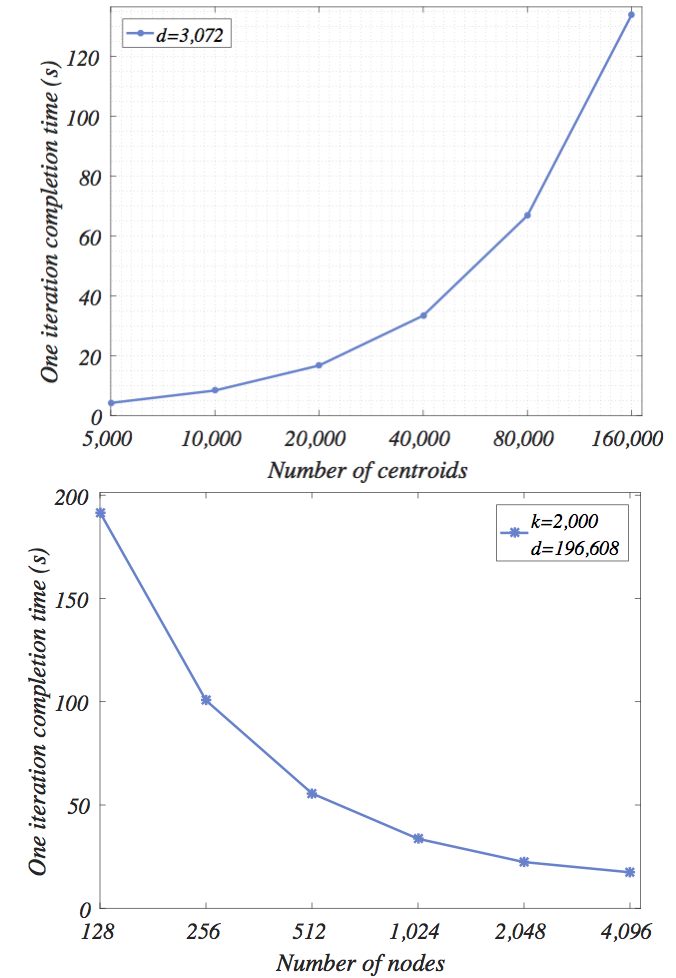
\includegraphics[scale=0.50]{scale.png}
\caption{Level 3 - large-scale on centroids and nodes}
\label{scale}
\end{figure}

\begin{figure}
\centering
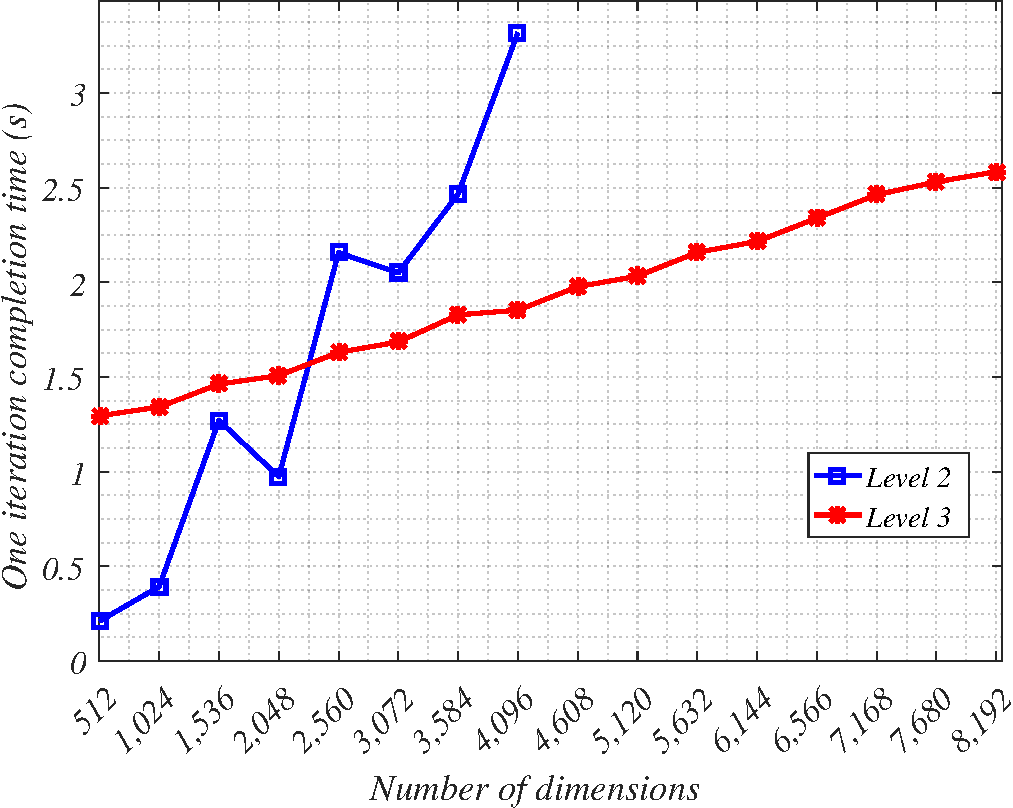
\includegraphics[scale=0.3]{sd.pdf}
\caption{Comparison: varying d with 2,000 centroids and 1,265,723 data samples tested on 128 nodes}
\label{sd}
\end{figure}

\begin{figure}
\centering
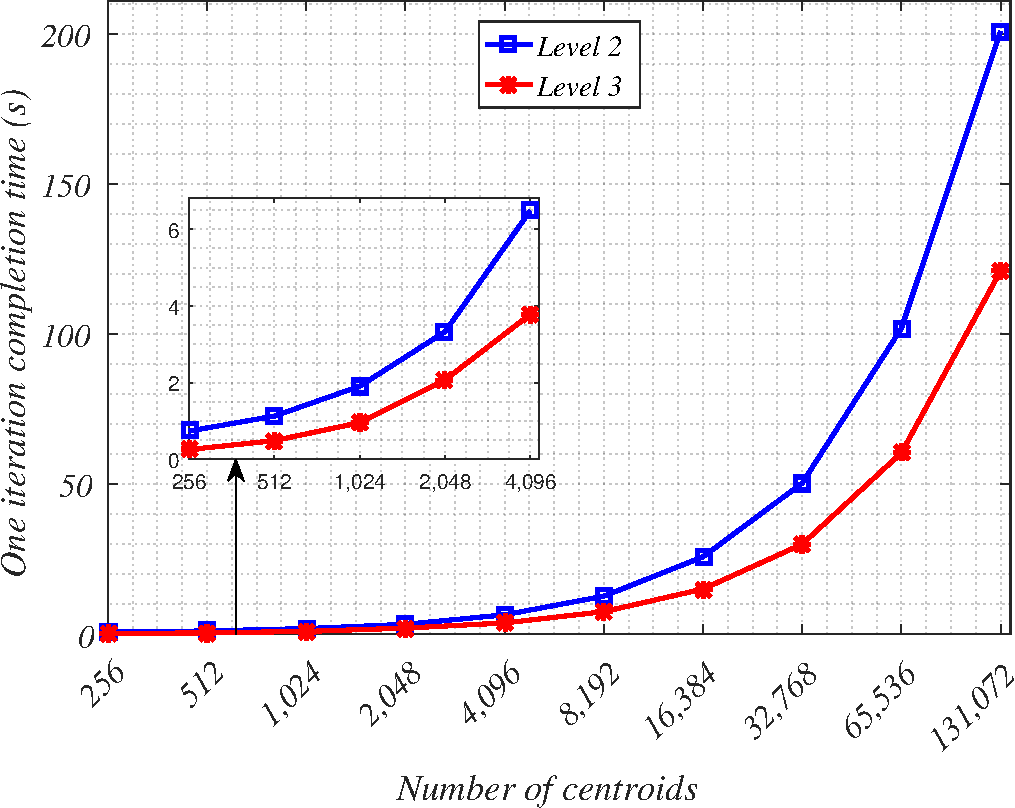
\includegraphics[scale=0.3]{sk.pdf}
\caption{Comparison test: varying k with 4,096 dimensions and 1,265,723 data samples tested on 128 nodes}
\label{sk}
\end{figure}

\begin{figure}
\centering
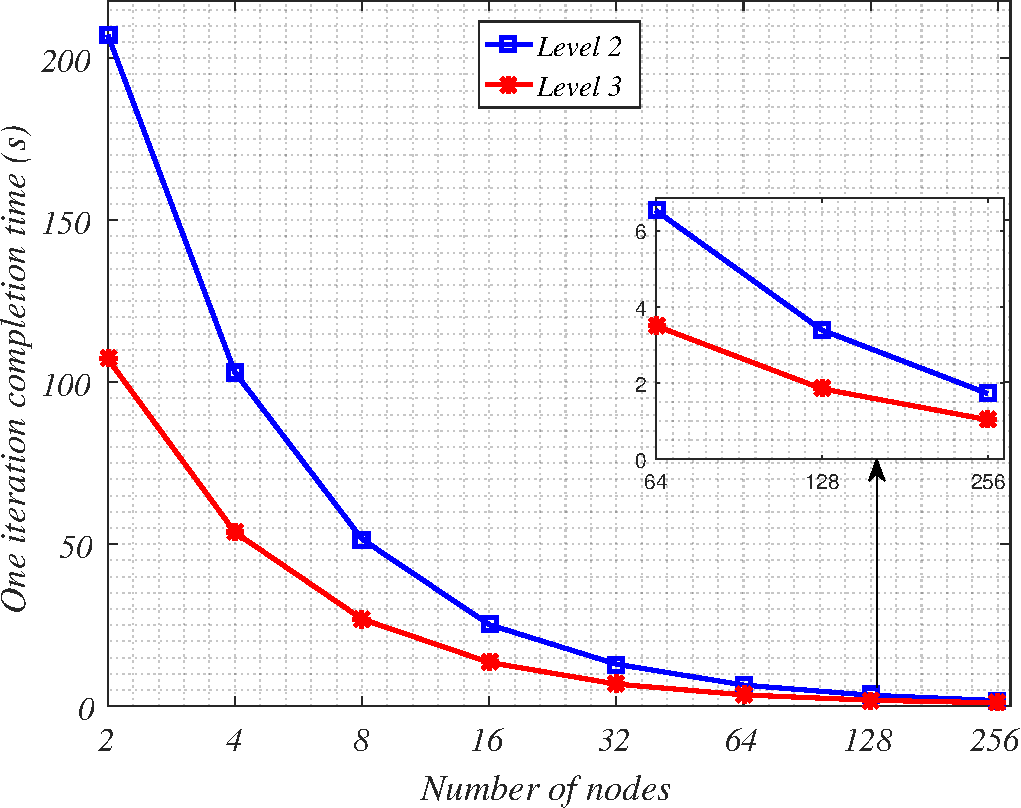
\includegraphics[scale=0.3]{sn.pdf}
\caption{Comparison test: varying number of nodes used with a fixed 4,096 dimension, 2,000 centroids and 1,265,723 data samples}
\label{sn}
\end{figure}

\subsubsection{Comparison of partition levels}

In this section we experimentally compare the \textit{Level 2} approach with \textit{Level 3}.

Figure \ref{sd} shows how {\it one iteration completion time} grows as the number of dimensions increases. The Level 2 approach outperforms Level 3 when the number of dimensions is relatively small. However, the Level 3 approach scales significantly better with growing dimensionality, outperforming Level 2 for all $d$ greater than 2560.  The Level 2 approach cannot run with $d$ greater than 4096 in this scenario due to memory constraints. However, it is clear that, even if this problem were solved, the poor scaling would still limit this approach. The completion time for Level 2 falls twice unexpectedly between 1536 and 2048, and between 2560 and 3072. This is due to the crossing of communication boundaries in the architecture of the supercomputer -- the trend remains clear however.

Figure \ref{sk} shows how the {\it one iteration completion time} grows as the number of centroids, $k$ increases. Since the number of $d$ is fixed at 4096, the Level 3 approach actually always outperforms Level 2, with the gap increasing as $k$ increases. This scaling trend is replicated at lower levels of $d$ too, though Level 2 initially outperforming Level 3 at lower values of $k$.

Figure \ref{sn} shows how both Level 2 and Level 3 scale across an increasing number of computation nodes. Level 3 clearly outperforms Level 2 in all scenarios. The values of $k$ and $d$ are fixed, as described in the graph caption, at levels which Level 2 can operate. The performance gap narrows as more nodes are added, but remains significant. Clearly the exact performance numbers will vary with other values $k$ and $d$, as can be inferred from other results, but the main conclusion we draw here is that Level 3 generally scales well.

%To further demonstrate the advantage of multi-level approach, we design a comparison experiment to test between level 3 and level 2. In this experiment, we use {\it ILSVRC2012} dataset from ImgNet with 265,723 samples. To show the results by varying $d$, we setup nodes to be 128, $k$ to be 2,000 and results is in Figure \ref{sd}; To show the results by varying $k$, we setup nodes to be 128, $k$ to be 4,096 and results is in Figure \ref{sk}; To show the results by cross number of nodes, we setup $d$ to be 4,096, $k$ to be 2,000 and results is in Figure \ref{sn}.

%As can be found in this graph, the level 3 design keeps performing better  than level 2 design when either varying $k$ or number of nodes in this comparable setting. A nearly linear speedup can be achieved for both designs. More interesting results are shown in the figure for varying $d$: Level 2 design is better than level 3 when $d$ is less than 2,560 which demonstrate the flexibility of the multi-level approach. When $d$ is greater or equal to 2560, level 3 begins to show advantage on performance from the fully data partition. Then as the $d$ continually increased to more than 4096, level 2 design without an efficient data partition method failure to finish the job anymore, while the level 3 design can still enjoy a super linear speedup. This results confirm the target high-performance and flexibility of our multi-level scalable design on vary workload sizes. 

\subsubsection{Comparison with other architectures}

\begin{table*}
  \caption{Execution time comparison with other architectures}
  \center
  \label{ccpu}
   \begin{tabular}{p{2cm} p{3.2cm} p{1cm} p{1cm}p{0.5cm}p{2cm}p{3cm}p{1cm}p{1cm} c c c c c c c }
 % \begin{tabular}{l c c c c}
    \hline
    Approaches&Hardware Resources &n & k & d& Execution time per iteration (sec.) & Execution time per iteration by Sunway TaihuLight (sec.) & Max. Speedup\\
    \hline
    Rossbach, et al\cite{rossbach2013dandelion} &10x NVIDIA Tesla K20M + 20x Intel Xeon E5-2620&1.0E9 &120 &40 &49.4&0.468635 (128 nodes) & 105x\\
      \hline
    Bhimani, et al\cite{bhimani2015accelerating} &NVIDIA Tesla K20M&1.4E6 &240 &5 &1.77&0.025336 (4 nodes) & 70x\\
      \hline
    Jin, et al\cite{jin2018high} &NVIDIA Tesla K20c&1.4E5&500&90&5.407&0.110191 (1 node) & 49x\\ 
    %li, et al\cite{li2010speeding}&NVIDIA GTX280&8.19E8 &100 &34&3098&35.644107  \\
      \hline
    Li, et al\cite{li2016high}&Xilinx ZC706&2.1E6&4&4&0.0085&0.002839 (1 node) & 3x\\
      \hline
    Ding, et al\cite{ding2015yinyang} &Intel i7-3770K&2.5E6 &10,000 &68 &75.976&2.424517 (16 nodes) & 31x\\
%      \hline
%    Wang, et al\cite{wang2014optimising} \\

%    ILSVRC2012 &8.1E6 &1000 &4096 \\
%    RCV1 &1.9E5 &103 &1979  \\
    \hline
  \end{tabular}
\end{table*}

As discussed, state-of-the-art supercomputing-oriented approaches are tested either on their specific datasets \cite{kumar2011parallel,cai2015grouping} or publish only their relative speedups \cite{bender2015k} instead of execution times. It is not possible to compare our actual execution time with these supercomputing-oriented approaches directly. Additionally, wallclock execution times are problematic to compare across vastly differing architectures with different budgets.

To give some insight into the performance we obtain, we compare execution time with other architectures directly where this is possible. We present five comparable results from published literature in Table \ref{ccpu}. Based on the differing workload sizes presented in these papers, we adjust the hardware configuration for Sunway TaihuLight, changing the number of nodes utilized. This is determined by the size of the task in terms of $k$ and $d$ where no further performance gains are possible by adding more nodes. The number of nodes varies from just one node for a single processing unit \cite{jin2018high,li2016high} to 128 nodes in \cite{rossbach2013dandelion}.
We report results against a heterogeneous node based approach running a custom implementation of parallel k-means on ten heterogeneous nodes, each node consisting of an NVIDIA Tesla K20M GPU with two Intel Xeon E5-2620 CPUs \cite{rossbach2013dandelion}. Further, we compare against two GPU based implementations  running on an NVIDIA Tesla K20M GPU and an NVIDIA Tesla K20C GPU respectively \cite{bhimani2015accelerating, jin2018high}, an FPGA based approach running a custom parallel k-means implementation on Xilinx ZC706 FPGA \cite{li2016high}, and a multi-core processor based approach running a custom implementation of parallel k-means on 8-core Intel i7-3770k processor \cite{ding2015yinyang}.
%The first one is a multi-core processor based experiment -- this work ran a custom implementation of parallel k-means on 8-core Intel i7-3770k processor with 16 GB memory targeting on 3 datasets from UCI machine learning repository\cite{uci}, published in \cite{ding2015yinyang}. 
%The second is a GPU based experiment -- this work runs a custom parallel k-means implemtnation on NVIDIA GTX280 GPU targeting on the KDD Cup 1999 dataset\cite{kdd}, which was published in \cite{li2010speeding}.

The proposed approach running on the Sunway TaihuLight supercomputer achieves more than $100$x speedup over the high-performance heterogeneous nodes based approach, between $50$x-$70$x speedup than those single GPU based approaches, and $31$x speedup over multi-core CPU based approach on their largest solvable workload sizes. 

%nearly $20$x speedup than the Intel multi-core processor based approach and nearly $100$x speedup than the NVIDIA GPU based approach on their largest solvable workload sizes. 

%commented by zwl for camera ready
%Although we are able to show substantial improvement against these architectures, the approach presented in this paper is principally designed for, and performs best on higher dimensionality and higher numbers of centroids than is possible on such small systems.


\subsection{Impact on Applications}\label{applications}

\begin{figure}
\centering
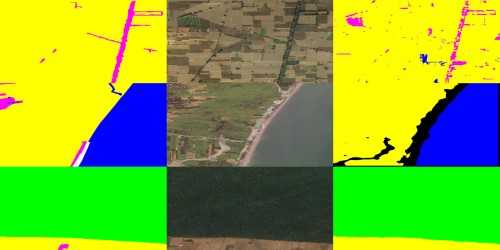
\includegraphics[scale=0.40]{lc1.jpg}
\caption{Remote Sensing Image Classification. Left: the result from baseline approach provided by \cite{demir2018deepglobe}. Middle: the corresponding original image. Right: our classification result. 
%We apply different colors to identify different region classes as used in \cite{demir2018deepglobe}.
}
\label{lc}
\end{figure}

As a widely used clustering algorithm, a highly efficient and scalable $k$-$means$ implementation is important to support applications with increasingly large problem sizes and data processing requirements. 
To demonstrate the efficacy of our design on real applications, we report results for the \textit{land cover classification} application and the \textit{gene expression data classification} application. 

\subsubsection{Land Cover Classification}
This is a popular remote sensing problem, requiring unsupervised methods to handle high numbers of unlabeled remote sensing images \cite{li2016stacked}.
$K$-$means$ has already been used for regional land cover classification with small number of targeted classes. For example, Figure \ref{lc} shows our result of classifying a remote sensing image (from a public dataset called Deep Globe 2018 \cite{demir2018deepglobe}) into 7 classes, representing the urban, the agriculture, the rangeland, the forest, the water, the barren and unknown. There are 803 images in the Deep Globe 2018 dataset, and each image has about $2k \times 2k$ pixels. The resolution of the image is 50cm/pixel. In this problem definition, we cluster on one image, where $n$ is 5838480, $k$ is 7 and $d$ is 4096, which can be done with 400 SW26010 many-core processors. Our Level 3 design can process the clustering dataset efficiently. 
%Furthermore, the Level 2 design can support classification with more classes (such as urban area and polar regions) and enables more sub-classes (such as different kinds of vegetation). 
In recent years, high-resolution remote sensing images have become more common in land cover classification problems. The problem definition on high-resolution images is more complex as the classification sample can be a block of pixels instead of one pixel, which means the $d$ can be even larger.
%For example, if we  choose a $30m \times 30m$ area as a sample, there are $30\times30$ pixels and $d$ is 5400, which can be efficiently supported by our Level 3 design. 

Real world research of high-resolution land cover classification and other similar problems are currently in progress on the Sunway TaihuLight supercomputer, using the method proposed in this paper. 

%Further significant applications with intrinsic high dimensionality are potentially supported.
\subsubsection{Gene Expression Data Classification}
Genomic information from gene expression data has been widely used and already benefited on improving clinical decision and molecular profiling based patient stratification. Clustering high-dimensional gene expression data on HPC with efficient parallel processing has achieved high performance on stratifying subjects and building classifiers \cite{wang2014optimising}. 

To demonstrate the advantage from our large-scale $k$-$means$ algorithm on Sunway TaihuLight supercomputer targeting this application, we test on the same datasets (MULTMYEL) \cite{genedata} with the previous work \cite{wang2014optimising} and compare the performance. There are 559 subjects and each subject has 54675 probesets. In this problem definition, we cluster the whole dataset, where $n$ is 559, $d$ is 54675 and $k$ is from 5 to 80 (the range tested on the previous work). The previous work applied hierarchical clustering and run on 32 CPU cores by a single VM, while our approach applies our level-3 partitioning and run a single CG with 64 CPEs. The performance of our approach against this work is shown in figure~\ref{compare_g}. We present the performance on execution time on difference number of centroids. We achieve a dramatic speedup on total execution time from 198x on $k$=5 to up-to 18000x on $k$=80. 

We further apply the auto-clustering evaluation function to determine the optimal value of $k$. The results is shown in figure~\ref{}.

\begin{figure}
\centering
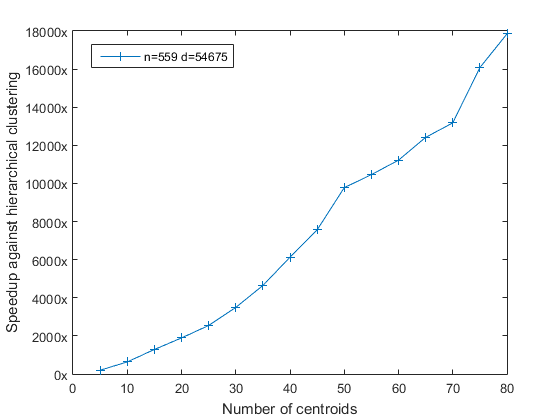
\includegraphics[scale=0.50]{compare.png}
\caption{ Speedup on total execution time for gene expression dataset MULTMYEL \cite{genedata} against a previous hierarchical clustering approach \cite{wang2014optimising}.
}
\label{compare_g}
\end{figure}

\section{Conclusions}
This paper presents the first ever fully data partitioned ($nkd$-partition) approach for parallel $k$-$means$ implementation to achieve scalability and high performance at large numbers of centroids and high data dimensionality simultaneously. Running on the Sunway TaihuLight supercomputer, it breaks previous limitations for high performance parallel $k$-$means$, allowing data scientists a new powerful tool with great potential.

The proposed multi-level approach also achieves greater flexibility on general workloads with varying data size, target centroids and data dimensions compared with previous supercomputer-specific approaches.  The novel design unlocks the potential of hierarchical hardware support of the Sunway TaihuLight for $k$-$means$, and shows how to optimize this and potentially similar algorithms for a cutting edge heterogeneous many-core supercomputer design.


%\section*{Acknowledgment}
%H.Fu is supported by National Key R\&D Program of China (Grant No. 2017YFA0604500), by National Natural Science Foundation of China (Grant No. 91530323, 5171101179).

%L.Li is supported by by the National Natural Science Foundation of China (Grant No. 61702297), by China Postdoctoral Science Foundation (grant no. 2016M601031).

%J.Thomson and T.Yu are supported by the EPSRC grants "Discovery" EP/P020631/1, "ABC: Adaptive Brokerage for the Cloud" EP/R010528/1, and EU Horizon 2020 grant TeamPlay: "Time, Energy and security Analysis for Multi/Many-core heterogenous PLAtforms" (ICT-779882, https://teamplay-h2020.eu).

%G.Yang is supported by the National Key R\&D Program of China (Grant No. 2016YFA0602200).

%W.Zhao is supported by the National Key R\&D Program of China (Grant No. 2017YFB0202204).

\bibliographystyle{plain}
\bibliography{acmart.bib}





%Appendix A
%\section{Register Communication}
%We usually perform a general matrix-matrix multiplication (GEMM) operation on data without SW26010 architecture. Register communication mechanism inside the 8*8 CPEs mesh, which is designed for supporting data transfer between 8 CPEs within the same row/column, is an unique feature of the SW26010 architecture. We can use register communication to optimization LDM-GEMM.

%In the 8 by 8 CPE mesh, the data exchange channels are formed by \emph{row communication buses} and \emph{column communication buses}. We achieve register-level communication by a pair of \emph{Put} and \emph{Get} operations through \emph{row/column communication buses}. The sender CPE send a 256-bit register file to the \emph{Transfer Buffer} of a receiver CPE by performing the \emph{Put} operation, while the receiver CPE fetch the 256-bit data from the \emph{Transfer Buffer} to the local general-purpose register file by performing the \emph{Get} operation. To ensure multi-Put and multi-Get operations, we implement a producer-consumer strategies. In addition, SW26020 also provides mechanisms to broadcast and multicast 256-bit data items.
%In the basic case, We need to apply register communication mechanism to update centroids in the second step. After finding the minimum distance from each sample to all centroids and identifying the cluster each sample should be attached 

%As for K-means algorithm based on Sunway architecture, CPEs need to communicate with each other for the next calculation. For the rows, each CPE can get computational results from the \emph{Transfer Buffer} of the rest 7 CPEs by performing the \emph{Get} operation. In addition, each CPE also send the computational result to the \emph{Transfer Buffer} of the rest 7 CPEs by performing the \emph{Put} operation, thus each CPE can get computational results from their own rows and sum them. CPEs have similar operations in the same column. Finally, each CPE has the count of all computational results after row communication and column communication.
%Formalized, we use CPE(ro,co) to index the 64 CPEs, and use $res_{ro co}$ to denote the res belonged to each CPE. To formalize the steps, we obtain:
%$$CPE(ro,co) \leftarrow \sum^{7}_{ro=1}(res_{ro co})$$
%$$CPE(ro,co) \leftarrow \sum^{7}_{co=1}(res_{ro co})$$
% This next section command marks the start of
% Appendix B, and does not continue the present hierarchy












\end{document}


